
%\documentclass[a4paper,UKenglish,cleveref, autoref, thm-restate,authorcolumns]{lipics-v2019}
\documentclass[a4paper,UKenglish,cleveref, autoref, thm-restate,authorcolumns]{../lipics/lipics-v2019}

%This is a template for producing LIPIcs articles. 
%See lipics-manual.pdf for further information.
%for A4 paper format use option "a4paper", for US-letter use option "letterpaper"
%for british hyphenation rules use option "UKenglish", for american hyphenation rules use option "USenglish"
%for section-numbered lemmas etc., use "numberwithinsect"
%for enabling cleveref support, use "cleveref"
%for enabling autoref support, use "autoref"
%for anonymousing the authors (e.g. for double-blind review), add "anonymous"
%for enabling thm-restate support, use "thm-restate"

%\graphicspath{{./graphics/}}%helpful if your graphic files are in another directory

\usepackage{amsmath} % provides many mathematical environments & tools
\usepackage{amsthm}
\usepackage{amssymb}
\usepackage[usenames,dvipsnames]{xcolor}
\usepackage{textcomp}
\usepackage{pgf}
\usepackage{pgfgantt}
\usepackage{pgfplots}\pgfplotsset{compat=1.3}
\usepackage{setspace}
\graphicspath{{../lipics/plots/}}
%\usepackage[colorlinks,linkcolor=ForestGreen,citecolor=ForestGreen]{hyperref}
%\usepackage[hidelinks]{hyperref}
%\usepackage[nameinlink, capitalize]{cleveref} %used for cross theorem references
%\setlength{\parindent}{5mm}
%\usepackage[english]{babel}
%\usepackage{verbatim}
\usepackage[normalem]{ulem} %for strikethrough text

\usepackage{qtree}
\usepackage[dvipsnames]{xcolor}

\usepackage{tikz}%used for examples for problems in earlier analysis

\usepackage{algorithm}
\usepackage{algorithmic}

\usepackage{tabularx,ragged2e}%used for tables with long text in some columns
\newcolumntype{C}{>{\arraybackslash}X}%column type that supports long texts, i.e. text across multiple lines
\setlength\extrarowheight{3pt}


% !TeX spellcheck=en_GB

\newcommand{\R}{\mathbb{R}}
\newcommand{\nl}{\newline}
\newcommand{\blue}[1]{\textcolor{blue}{#1}}
\newcommand{\red}[1]{\textcolor{purple}{#1}}

\newcommand{\adjDel}{\textsc{pCrep}}
\newcommand{\static}{\textsc{Static}}
\newcommand{\adapt}{\textsc{Adapt}}
\newcommand{\directDecomp}{\textsc{dCrep}}

\newcommand{\size}{\text{\scriptsize SIZE}}
\newcommand{\optmig}{\text{\scriptsize OPT-MIG}}
\newcommand{\optreq}{\text{\scriptsize OPT-REQ}}
\newcommand{\del}{\text{\scriptsize DEL}}
\newcommand{\ovr}{\text{\scriptsize OVR}}
\newcommand{\final}{\text{\scriptsize FINAL}}
\newcommand{\opt}{\text{O{\scriptsize PT}}}
\newcommand{\alg}{\text{A{\scriptsize LG}}}
\newcommand{\core}{\text{\scriptsize CORE}}
\newcommand{\halo}{\text{\scriptsize HALO}}
\newcommand{\req}{\text{\scriptsize REQ}}
\newcommand{\finalComps}{\text{\scriptsize FIN-COMPS}}
\newcommand{\finalWeights}{\text{\scriptsize FIN-WEIGHTS}}
\newcommand{\epoch}{\text{\scriptsize EPOCH}}
\newcommand{\delTime}{\text{\scriptsize DEL-TIME}}
\newcommand{\reqTime}{\text{\scriptsize TIME}}
\newcommand{\comps}{\text{\scriptsize COMPS}}
\newcommand{\onl}{\text{O{\scriptsize NL}}}
\newcommand{\coreDel}{\text{C{\scriptsize REP}-C{\scriptsize ORE}}}


\newcommand{\dbALong}{Mocfe}
\newcommand{\dbBLong}{NeckBone}
\newcommand{\dbCLong}{MultiGrid}
\newcommand{\fbLong}{Facebook}

\newcommand{\dbA}[0]{Mocfe}
\newcommand{\dbB}{NB}
\newcommand{\dbC}{MG}
\newcommand{\fb}{FB}
\newcommand{\dbmocfe}{Mocfe}
\newcommand{\dbnekbone}{NB}

\newcommand\stefan[1]{{\color{blue}\textbf{Stefan: #1 }}}

\newcommand{\new}[1]{{\textcolor{blue}{#1}}}
\newcommand{\old}[1]{{\text{\textcolor{red}{\sout{#1}}}}}

%commands for input sequence diagrams
\newcommand{\request}[3]{\draw (axis cs:#3,#1) -- node[left]{} (axis cs:#3,#2);}

\bibliographystyle{plainurl}% the mandatory bibstyle

\title{Online Balanced Repartitioning 
of Dynamic Communication Patterns in Polynomial Time} %TODO Please add

\titlerunning{Polytime Online Repartitioning} %TODO optional, please use if title is longer than one line

\author{Anonymous Submission}{\#127}{}{}{}

%\author{Tobias Michael Forner}{Technical University of Munich, Germany}{}{}{}%TODO
%\author{Harald Räcke}{Technical University of Munich, Germany}{}{}{}%TODO
%\author{Stefan Schmid}{Faculty of Computer Science, University of Vienna, Austria}{}{}{}%TODO

\authorrunning{Submission \#127}

%\authorrunning{Forner et al.} %TODO mandatory. First: Use abbreviated first/middle names. Second (only in severe cases): Use first author plus 'et al.'

\Copyright{} %TODO mandatory, please use full first names. LIPIcs license is "CC-BY";  http://creativecommons.org/licenses/by/3.0/

\begin{CCSXML}
<ccs2012>
   <concept>
       <concept_id>10003752.10003809.10010047</concept_id>
       <concept_desc>Theory of computation~Online algorithms</concept_desc>
       <concept_significance>500</concept_significance>
       </concept>
   <concept>
       <concept_id>10010520.10010521.10010537</concept_id>
       <concept_desc>Computer systems organization~Distributed architectures</concept_desc>
       <concept_significance>500</concept_significance>
       </concept>
 </ccs2012>
\end{CCSXML}

\ccsdesc[500]{Theory of computation~Online algorithms}
\ccsdesc[500]{Computer systems organization~Distributed architectures}

\keywords{Online algorithms, graph partitioning, migration, competitive analysis} %TODO mandatory; please add comma-separated list of keywords

\category{} %optional, e.g. invited paper

\relatedversion{} %optional, e.g. full version hosted on arXiv, HAL, or other respository/website
%\relatedversion{A full version of the paper is available at \url{...}.}

\supplement{}%optional, e.g. related research data, source code, ... hosted on a repository like zenodo, figshare, GitHub, ...

%\funding{(Optional) general funding statement \dots}%optional, to capture a funding statement, which applies to all authors. Please enter author specific funding statements as fifth argument of the \author macro.
%TODO add acknowledgements
%\acknowledgements{Research supported by
%ERC Consolidator grant No. 864228 (AdjustNet). 
%}%optional

\nolinenumbers %uncomment to disable line numbering

\hideLIPIcs  %uncomment to remove references to LIPIcs series (logo, DOI, ...), e.g. when preparing a pre-final version to be uploaded to arXiv or another public repository

%Editor-only macros:: begin (do not touch as author)%%%%%%%%%%%%%%%%%%%%%%%%%%%%%%%%%%
\EventEditors{John Q. Open and Joan R. Access}
\EventNoEds{2}
\EventLongTitle{42nd Conference on Very Important Topics (CVIT 2016)}
\EventShortTitle{CVIT 2016}
\EventAcronym{CVIT}
\EventYear{2016}
\EventDate{December 24--27, 2016}
\EventLocation{Little Whinging, United Kingdom}
\EventLogo{}
\SeriesVolume{42}
\ArticleNo{23}
%%%%%%%%%%%%%%%%%%%%%%%%%%%%%%%%%%%%%%%%%%%%%%%%%%%%%%

\begin{document}

\maketitle

%TODO mandatory: add short abstract of the document
\begin{abstract}
This paper revisits the online balanced repartitioning problem
(introduced by Avin et al. at DISC 2016) which asks for a scheduler
that dynamically collocates frequently communicating nodes,
in order to reduce communication costs 
while minimizing migrations in distributed systems. 
More specifically, communication requests arrive online and 
need to be served, either remotely across different servers at cost 1, 
or locally within a server at cost 0; before serving a 
request, the online scheduler 
can change the mapping of nodes to servers, i.e., migrate nodes, 
at cost $\alpha$ per node move.
Avin et al. presented a deterministic \new{$O(k \log k)$}\old{$O(n \log n)$}-competitive
algorithm, which is optimal
up to a logarithmic factor; however, their algorithm has the drawback
that it relies on expensive repartitioning operations which result in
a super-polynomial runtime.
Our main contribution is a different deterministic algorithm $\adjDel$ 
which achieves the same
competitive ratio, but runs in polynomial time.  
Our algorithm monitors the connectivity of communication requests over time, rather than the density as in prior work; this enables 
the polynomial runtime. 
We analyze $\adjDel$ both
analytically and empirically.
\end{abstract}

\pgfplotstableread[row sep=\\,col sep=&]{
	database & AdjDel 		& CoreDel & Adaptive & Static            \\
	\dbA		 & 142317.400000	& 153223	& 254994.20000  & 54919.400000 \\
	\dbB		 & 224418.600000 & 313985.600000 & 263278.400000 & 57454.200000 \\
	\dbC 		 & 229010.000000 & 295830.800000 & 173940.200000 & 14950.400000 \\
	%D		 & 100			 & 80 			 & 50			\\
}\totalcostplot

%communication cost
\pgfplotstableread[row sep=\\,col sep=&]{
	database & AdjDel 		& CoreDel 			& Adaptive 	& Static	\\
	\dbA		 & 54956.200000	& 55375.2		 & 93641.000000 & 48947.000000	\\
	\dbB		 & 109548.600000 & 119710.400000 & 56231.600000 & 51519.000000	\\
	\dbC		 & 100612.400000 & 110112.800000 & 59455.400000 & 9242.000000	\\
	%D 		 & 100			 & 80 			& 50			\\
}\commcostplot

%migration cost
\pgfplotstableread[row sep=\\,col sep=&]{
	database & AdjDel & CoreDel & Adaptive 	 & Static 		\\
	\dbA		 & 87361.200000 & 97848		 & 161353.200000 & 5972.400000	\\
	\dbB		 & 114870.000000 & 194275.200000 & 207046.800000 & 5935.200000	\\
	\dbC		 & 128397.600000 & 185718.000000 & 114484.800000 & 5708.400000	\\
	%D		 & 100			 & 80 			 & 50			\\
}\migcostplot

%running time in ms
\pgfplotstableread[row sep=\\,col sep=&]{
	database & AdjDel & CoreDel 	& Adaptive		& Static		\\
	\dbA		 & 48384.000000 & 102254			& 61374.6 		& 2588.399902	\\
	\dbB		 & 106468.000000 &622934.000000	& 32851.800781	& 2489.399902	\\
	\dbC		 & 131988.796875 & 428089.812500	& 42036.601562	& 2460.399902	\\
	%D 		 & 100				& 80 			& 50			\\
}\runtimeplot

%plots for coreDel and adjDel where only 2*alpha-connected components are merged

\pgfplotstableread[row sep=\\,col sep=&]{
	database & AdjDelDouble & CoreDelDouble 	\\
	\dbA		 & 111687.200000 & 124514.600000	\\
	\dbB		 & 156627.400000 & 187898.200000	\\
	\dbC		 & 153176.600000 & 192994.000000	\\
}\totalcostplotTwoAlpha

\pgfplotstableread[row sep=\\,col sep=&]{
	database & AdjDelDouble & CoreDelDouble 	\\
	\dbA		 & 44522.400000 & 54141.600000		\\
	\dbB		 & 50406.000000 & 77145.600000		\\
	\dbC		 & 51382.800000 & 81482.400000		\\
}\migcostplotTwoAlpha

\pgfplotstableread[row sep=\\,col sep=&]{
	database & AdjDelDouble & CoreDelDouble 	\\
	\dbA		 & 67164.800000 & 70373.000000		\\
	\dbB		 & 106221.400000 & 110752.600000	\\
	\dbC		 & 101793.800000 & 111511.600000	\\
}\commcostplotTwoAlpha

\pgfplotstableread[row sep=\\,col sep=&]{
	database & AdjDelDouble & CoreDelDouble 	\\
	\dbA		 & 72204.796875  & 175801.796875	\\
	\dbB		 & 141781.000000 & 948782.375000	\\
	\dbC		 & 396427.406250 & 938235.000000	\\
}\runtimeplotTwoAlpha

\section{Introduction}

Most distributed systems critically rely on an efficient
interconnecting communication network. With the 
increasing scale of these systems, the network traffic often grows accordingly:
applications related to distributed machine learning, 
batch processing, or scale-out databases, spend 
a considerable fraction of their runtime shuffling data \cite{Mogul2012}.
An interesting method to improve the efficiency in these 
systems is to exploit their resource allocation flexibilities:
many distributed systems are highly virtualized today and 
support to relocate (or migrate) communication partners (e.g. virtual machines).
By collocating two frequently communicating nodes on the same server,
slow and costly inter-server communication can be reduced.
However, relocations also come at a cost, and the number of migrations
should be kept low accordingly.

This paper revisits the online balanced repartitioning problem 
\cite{Avin2016} which models the tradeoff between the benefits
and the costs of dynamic relocations. The goal is to design an algorithm 
which maintains, at any time, a mapping of $n$ communication nodes (virtual machines) to $\ell$ servers of fixed equal size $k$; in the absence of augmentation,
$n=\ell k$. The communication pattern can be seen as a dynamic
graph, from which communication requests arrive in an online manner;
in other words, the online algorithm does not have prior knowledge of future communication requests. The goal is to strike a balance between the benefits
and the costs of migrations.
More specifically, the cost model is as follows: 
if a communication request is served remotely, i.e., between nodes mapped to different servers, it incurs a communication cost of 1;
communication requests between nodes located on the same server 
are free of cost. Before the cost for the current request is payed, an algorithm has the option to migrate nodes at a cost of $\alpha$ for each node move.

The problem can be seen as
a symmetric version of caching: two nodes can be ``cached''
together on any server.

\subsection{Contributions}

Our main result is a deterministic online algorithm \adjDel{}
for the dynamic balanced graph partitioning problem 
which achieves a competitive ratio of $O(k\log k)$
and runs in \emph{polynomial time}, for a constant augmentation. 

A $O(k\log k)$-competitive algorithm was already given by 
Avin et al. in \cite{Avin2016}, together with an almost tight lower bound
$\Omega(k)$. However, the algorithm relies on expensive repartitioning
which results in a super-polynomial runtime.   
Our algorithm, \adjDel{}, is similar to the algorithm by Avin et al.,
but it comes with a twist: rather than considering the \emph{density}
of emerging communication patterns when deciding the repartitioning,
we consider the \emph{connectivity}. The latter allows for polynomial-time
approximations, as we will show, but also requires a new analysis.

We not only evaluate our algorithm analytically but also in simulations,
based on real datacenter workloads. 
To this end, we also perform algorithm engineering and make 
slight adaptations of our algorithms in order to improve their results.
%We further present a second algorithm, \coreDel, 
%an efficient heuristic which serves us as a baseline for comparison,
%and which may be of independent interest. 
We will make our implementation publicly available as open source,
together with this paper.

\subsection{Preliminaries}

Let us introduce some 
definitions and notations 
that will be used throughout the paper.
We define a graph $G=(V, E, w)$ 
where $V$ is the set of vertices,
$E$ the set of (undirected) edges,
and $w:E \rightarrow \mathbb{N}$ assigns each edge an (integer) weight.
Given a graph $G=(V,E,w)$,
we define an \textit{(edge) cut} of $G$ as a pair of 
two disjoint subsets $X,Y$ of $V$ such that $X\cup Y=V$. 
The value of this cut is the sum of the weight of edges between 
nodes from $X$ and $Y$, i.e. $\sum_{e=\{u,v\}\in E:u\in X, v\in Y}w(e)$ is the value of the cut $(X,Y)$. Note that such a cut can also be defined by the set of the edges connecting $X$ and $Y$ that are cut. We call a cut a \textit{minimum (edge) cut} of $G$ if it is one of the cuts with minimum value.

The \textit{connectivity} of a graph $G$ is equal to the value of a minimum edge cut of $G$. This definition will be used in order to define the communication components our algorithm maintains as these are subsets of $V$ which induce subgraphs of high connectivity. We explain the concept of components in greater detail later.

Furthermore we define the term $(s,t)$\textit{-cut} as a cut $(X,Y)$ for which $s\in X$ and $Y\in X$, i.e. a $(s,t)$-cut separates the nodes $s$ and $t$ in $G$. Then a \textit{minimum $(s,t)$-cut} is a $(s,t)$-cut of minimum value. Note that a minimum $(s,t)$-cut is not necessarily a minimum cut.

Finally we call an injective function $m:X\rightarrow Y$ a \textit{mapping of $X$ to $Y$}. We use this terminology for example when we talk about the assignment of nodes to servers.

\sloppy

\section{Model}
\label{problem_definition_section}

We consider the problem of maintaining a partitioning of a 
set of $n=k\cdot \ell$ nodes (e.g., processes or virtual machines) 
that communicate with each other, 
into $\ell$ servers (henceforth sometimes also called clusters) of size $k$ each, 
while minimizing both the cost due to communication and due to node migrations. 
More formally we are given $\ell$ servers $V_0,...,V_{\ell-1}$, 
each with capacity $k$ and an initial perfect mapping of $n=k\cdot \ell$ nodes to the $\ell$ servers, 
i.e. each server is assigned exactly $k$ nodes. An input sequence $\sigma=((u_1, v_1),1), ((u_2, v_2),2),...()(u_i,v_i),i),...$ describes 
the sequence of communication requests: the pair $((u_t, v_t),t)$ represents a communication request between the nodes 
$u_t$ and $v_t$ arriving at time $t$. At time $t$ the algorithm is allowed to perform node migrations at a cost of $\alpha>1$ per move. 
After the migration step, the algorithm pays cost 1 if $u_t$ and $v_t$ are mapped to different servers and does not pay any cost otherwise. Note that an algorithm may also choose to perform no migrations at all.

We are in the realm of competitive analysis and as a result we compare an online algorithm \onl{} to the optimal offline algorithm \opt{}. \onl{} only learns of the requests in the input sequence $\sigma$ as they happen and as a result only knows about the partial sequence $(u_1,v_1),...,(u_t,v_t)$ at time $t$ whereas \opt{} has perfect knowledge of the complete sequence $\sigma$ at all times.

The goal is to design an online algorithm \onl{} with a good competitive ratio with regard to \opt{} defined as follows.
An online algorithm \onl{} is $\rho$-competitive if there exists a constant $\beta$ such that 
\begin{align*}
\onl{}(\sigma)\leq\rho\cdot \opt{}(\sigma)+\beta\:\forall \sigma
\end{align*} 
where $\onl{}(\sigma)$ and $\opt{}(\sigma)$ denote the cost of serving input sequence $\sigma$ of \onl{} and \opt{} respectively. \new{This has to hold for any input sequence $\sigma$.}

We consider a model with augmentation (as in prior work \cite{Avin2016}),
and allow the online algorithm to use larger capacities per server. 
In particular, the online algorithm is allowed to assign $(2+\epsilon)\cdot n/\ell$ nodes to each server where $\epsilon>0$. 
This augmented online algorithm is then compared with the optimal offline algorithm \opt{} which is not allowed to use any augmentation.

Throughout this paper, 
we will also use $1+\epsilon$ as the basis for the logarithm.

\section{Basic Algorithm}
\label{algIdeas}

We first describe the basic algorithm underlying
our approach, before presenting the polynomial-time implementation
later in this paper.
In general, \adjDel{} relies on a second-order partitioning of the communication nodes into \textit{communication components} which represent node-induced sub-graphs of the original communication graph given by the requests from the input sequence $\sigma$. \new{To this end we define a \textit{component} $C$ as the set of its nodes together with the time $t$ of its creation, i.e. $C=(\{v_1,v_2,...,v_k\}, t)$. For a component $B=(M, t)$ let $nodes(B)=M$, $\tau(B)=t$ and we define $|B|=|M|$ in order to improve readability}.
Initially each node forms a singleton component, but as the input sequence $\sigma$ is revealed, new communication patterns unfold. The algorithm keeps track of these patterns by maintaining a graph in which the nodes represent the actual communication nodes and the weighted edges represent the number of communication requests between nodes that were part of different components at the time of the request; that is, 
for edge $e=\{u,v\}$, $w(e)$ represents the number of paid communication requests between $u$ and $v$. We say that a communication request between nodes $u$ and $v$ is \textit{paid} if the nodes are located on different servers at the time of the request.
The algorithm merges a set $S$ of components into a new component $C$ if the connectivity of the component graph induced by the components in $S$ is at least $\alpha$. After each edge insertion the algorithm checks whether there exists a new component set $S$ with $|S|>1$ which fulfills this requirement.

If after any request and the insertion of the resulting edge the algorithm discovers a new subset $S$ of nodes whose induced subgraph has connectivity at least $\alpha$ and which is of cardinality at most $k$, it merges the components that form this set into one new component and collocates all the nodes in the resulting set on a single server. The algorithm reserves additional space $\min\{\lfloor\epsilon\cdot|C|\rfloor,k-|C|\}$ for each component \new{of size $|C|$} on the server it is currently located on. Note that the additional reservation may be zero for components smaller than $1/\epsilon$. This reservation guarantees that nodes are not migrated too often for the analysis to work. This also limits the total space a component can use to a maximum of $k$. This makes sense as a component whose size exceeds $k$ is deleted (rather than merged).
To this end the algorithms keep track of the reservations for each component.

The algorithm uses augmentation $2+\epsilon$ in order to guarantee that the collocation of such component sets of at most $k$ individual communication nodes is always possible without moving a node not in $C$. This guarantees by an averaging argument that there is always at least one cluster with capacity at least $k$, which a newly merged component can be moved to.

If the subset has cardinality greater than $k$, the resulting component is deleted.  
This general structure of our algorithm is also summarized in the form of pseudocode 
in \cref{highLevelAlg} and \cref{mergeAndRes}. 
In the pseudocode description we denote the reservation of a component $C$ by $res(C)$ and the current server it is mapped to by $serv(C)$. The free capacity of a server $i$ is denoted by $cap(i)$.

\begin{algorithm}[t]
	\caption{\adjDel{}}
	\label{highLevelAlg}
	\begin{algorithmic}
		\STATE \new{$G \gets (\{1,...,n\}, \emptyset, w)$ //\emph{initialize a graph on $n$ nodes without edges, $w$ assigns $0$ to every edge}} \old{initialize an empty graph on $n$ nodes}
		\STATE turn each of the $n$ nodes into a singleton component
		\FORALL{$r=\new{((u,v),t)}\old{\{u,v\}}\in\sigma$}
		
		\IF{$comp(v)\neq comp(u)$}
		\STATE $w(\{u,v\})\gets w(\{u,v\})+1$
		\ENDIF
		\IF{$\exists$ component set $X$ with connectivity at least $\alpha$ and $|X|>1$ and $nodes(X)\leq k$}
		\STATE mergeAndRes($X$)
		\ENDIF
		\IF{$\exists$ component set $Y$ with connectivity at least $\alpha$ and $nodes(Y)> k$}
		\STATE delete($Y$) // \emph{to be specified later} 
		\ENDIF	
		
		\ENDFOR
		
	\end{algorithmic}
\end{algorithm}

\begin{algorithm}[t]
	\caption{mergeAndRes($X$)}
	\label{mergeAndRes}
	\begin{algorithmic}
		\FORALL { $C\in X$}
		\STATE $cap(serv(C))\gets cap(serv(C))+res(C)$		
		\ENDFOR
		\STATE $N\gets collocate(X)$  // \emph{moves all components from $X$ to the same server as described} 
		\STATE // \emph{$N$ contains the newly created component} 
		\IF {$|N|>2/\epsilon$}
		\STATE // \emph{reserve additional space} 
		\STATE $res(N)\gets\min\{\lfloor\epsilon\cdot|N|\rfloor,k-|N|\}$
		\STATE $cap(serv(N))\gets cap(serv(N))-res(N)$
		\ENDIF	
		
		
	\end{algorithmic}
\end{algorithm}

 The main differentiating factor of this approach compared
to prior work \cite{Avin2015,Avin2016} is that we merge once a 
component set reaches connectivity $\alpha$, while prior approaches do so once the component set reaches a certain density threshold. More specifically earlier algorithms
 merge a component set $S$ once it fulfills $w(S)\geq(|S|-1)\cdot\alpha$ where $w(S)$ denotes the cumulative weight of the edges between nodes contained in the components of $S$.

\begin{algorithm}
	\caption{delete($Y$) of \adjDel{}}
	\label{adj_del_alg}
	\begin{algorithmic}
		\FORALL{$e=\{u,v\}\in E$}
		\IF{$u\in Y$ or $v\in Y$}
		\STATE $w(e)\gets0$
		\ENDIF
		\ENDFOR
		\FORALL{$C\in Y$}
		\STATE $cap(serv(C))\gets cap(serv(C)) +res(C)$
		\STATE $res(C)\gets 0$			
		\ENDFOR
	\end{algorithmic}
\end{algorithm}

\begin{algorithm}
	\caption{collocate($X$)}
	\label{alg:collocate}
	\begin{algorithmic}
		\STATE $C_{merged}\gets\bigcup_{C\in X} C$
		\IF{$\exists C\in X$ s.t. $res(C)>= |C|-|X|$}
		\STATE move all nodes to the server of $C$, freeing reservations and capacity
		\STATE $res(C_{merged})\gets res(C)-(|C_{merged}|-|C|)$
		\ELSE
		\STATE $target\gets$ $server$ s.t. $cap(server)\geq \min\{k, (1+\epsilon)|C_{merged}|\}$
		\STATE move all nodes from $X$ to $server$, freeing reservations and capacity
		\STATE $cap(server)\gets cap(server)-\min\{k, (1+\epsilon)|C_{merged}|\}$
		\STATE $res(C_{merged})\gets\min\{k, \epsilon|C_{merged}|\}$
		\ENDIF
	\end{algorithmic}
\end{algorithm}

\adjDel{} resets all the edges contained in the deleted component $C$ and also resets the 
weights of edges \textit{adjacent} to $C$, i.e. all edges $e=\{u,v\}$ are reset to zero 
if $u$ or $v$ were contained in component $C$ at the time of its deletion. The deletion
method is also described in pseudocode in \cref{adj_del_alg}.
Additionally, \cref{alg:collocate} describes the collocation procedure that first tries 
to find a component such that the remaining ones that are to be merged fit into its 
existing reservation (if-case). If this is not possible all the components that are to 
be merged are moved to a new server with enough space for the resulting merged component 
$C_{merged}$ as well as the additional reservation of $\min\{k, \epsilon|C_{merged}|\}$.
Furthermore the merge and deletion process is illustrated in \cref{exOldCrep}.

As we will see, the idea for the competitive analysis is to relate the cost of both \opt{} and \adjDel{} to the deleted components in the solution of \adjDel{}.
The fact that \adjDel{} also resets adjacent edges means that we can uniquely identify requests with the deleted component whose deletion led to the reset of the corresponding edge weights to zero. 

\begin{figure}
	\centering
	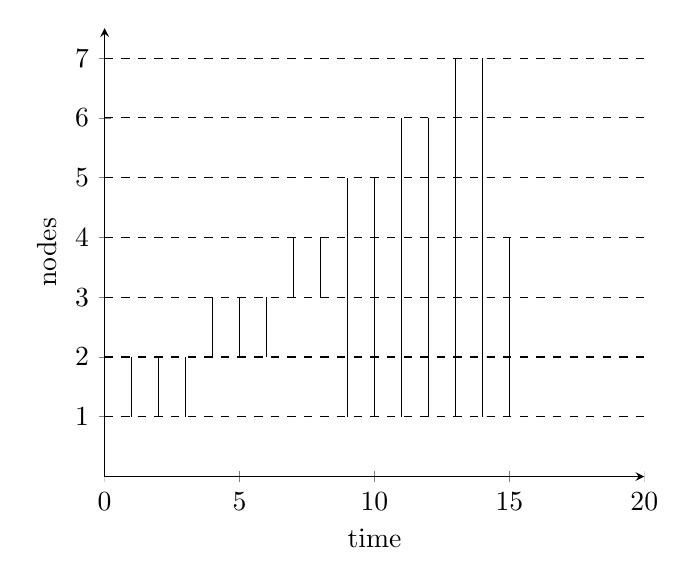
\begin{tikzpicture}
	\begin{axis}[xmin=0, xmax=20, ymin=0, ymax=7.5, axis lines=left, xlabel = time, ylabel = nodes, ytick = {1,2,3,4,5,6,7}]
	%nodes
	\addplot[domain=0:20, dashed] {1};
	\addplot[domain=0:20, dashed] {2};
	\addplot[domain=0:20, dashed] {3};
	\addplot[domain=0:20, dashed] {4};
	\addplot[domain=0:20, dashed] {5};
	\addplot[domain=0:20, dashed] {6};
	\addplot[domain=0:20, dashed] {7};
	
	%requests
	\request{1}{2}{1}
	\request{1}{2}{2}
	\request{1}{2}{3}
	\request{2}{3}{4}
	\request{2}{3}{5}
	\request{2}{3}{6}
	\request{3}{4}{7}
	\request{3}{4}{8}
	\request{1}{5}{9}
	\request{1}{5}{10}	
	\request{1}{6}{11}
	\request{1}{6}{12}
	\request{1}{7}{13}
	\request{1}{7}{14}
	\request{1}{4}{15}
	
	\end{axis}
	
	
	\end{tikzpicture}
	\caption{Illustration for the \adjDel{} approach: The horizontal lines represent the nodes over time, vertical lines represent request between the respective end points.  We consider the case where $\alpha=3$ and $k=3$.
	The first six requests lead \adjDel{} to merge the nodes \new{$\{1,2,3\}$}\old{$\{0,1,3\}$} into
	a new component $C$. The following eight requests connect the nodes 4, 5, 6 and 7 to $C$,
	but the respective cuts have value 2, hence no merge is performed. At time $t=15$ finally the node 4 gets merged with $C$ which results in a component of size 4 which gets deleted.
	During this deletion all edges shown in the figure are deleted, both those that led to the merges and the remaining ones.}\label{exOldCrep}
	
\end{figure}		

\section{Competitive Analysis}
\label{comp_analysis_section}

We analyze the competitive ratio of \adjDel{} with augmentation $(2+\epsilon)$ and show that \adjDel{} is $O(2/\epsilon\cdot k\log k)$-competitive.
We will use the following general definitions 
throughout the analysis.

\begin{definition}
	For any subset $S$ of components, let $w(S)$ be 
	the total weight of all edges between nodes of $S$.
\end{definition}

\begin{definition}
	We call a set of components of size at least 2 and of connectivity $\alpha$ 
	\textit{mergeable}.	
\end{definition}

\begin{definition}
	An $\alpha$\textit{-connected component} is a maximal set of vertices that is $\alpha$-connected.
\end{definition}

Despite the algorithmic differences, some claims
from \cite{Avin2015} can be adapted for \adjDel{}.
In Section \ref{sec:preli}, we introduce some preliminaries
which can easily be derived from prior work. 
In particular, we can show that there is always at most one mergeable component set after the insertion of a new edge which \adjDel{} then merges. The earliest point in time a new mergeable component set can emerge is after the next edge is inserted. 
In the following, we will now focus on the novel aspects of
the competitive analysis.

\subsection{Upper Bound On \adjDel{}}

We start the analysis with upper bounding the cost of \adjDel{} by introducing several notions that we will use throughout the analysis.
We define the set $\del(\sigma)$ as the set of components that were deleted by \adjDel{} during its execution given the input sequence $\sigma$.
We define the following notions for a deleted component $C\in\del{}(\sigma)$.
\new{
Let $\tau(v)$ be the time when the node $v$ was last turned into a singleton component and recall that $\tau(C)$ denotes the time at which component $C$ was created. Note that a component can either be created via merges or during the deletion process of another component $B$ when the nodes of $B$ are turned into singletons. If $C$ was one of the components created durung the initialisation of the algorithm then $\tau(C)=0$.}
Let $\epoch{}(C)$ denote the (node, time) pairs of nodes in $C$ starting at the time after the time $\tau(node)$ \old{when $node$ was last turned into a singleton component}, i.e. 
\begin{align*}
\epoch{}(C)=\bigcup_{\new{v}\old{n}\in nodes(C)}\{\new{v}\old{n}\}\times\{\tau(\new{v}\old{n})+1,...,\tau(C)\}.
\end{align*}

Note that for $C\in\del(\sigma)$, $\tau(C)$ denotes both the time of the creation as well as the time of deletion of $C$ \new{as $C$ is deleted by \adjDel{} right away}. We can use this definition of a component epoch $\epoch(C)$ to uniquely assign each node to a deleted component $C$ at each point in time $t$ (except for nodes in components that persist until the end of sequence $\sigma$).
We assign all requests to $\epoch(C)$ whose corresponding \new{edges} \old{requests} are deleted because of the deletion of component $C$ and call the set of those requests $\req(C)$.
We split the requests from $\req{}(C)$ into two sets: $\core(C)$ and $\halo(C)$. $\core(C)$ contains all requests for which both nodes have already been assigned to $C$ at the time of the request, i.e. 
\begin{align*}
\core(C)=\{r=\new{((u,v),t)}\old{\{u,v\}}\in\sigma| (u,\new{t}\old{\reqTime(r)})\in \epoch(C)\text{ and } (v, \new{t}\old{\reqTime(r)})\in \epoch(C)\}.
\end{align*}
These are the requests that led to the creation of component $C$ by increasing the connectivity within the corresponding subgraph.

We define $\halo(C)$ as the set of all requests from $\req(C)$ for which exactly one end point was associated with $C$ at the time of the request. Note that this means that $\halo(C)=\req(C)\backslash \core(C)$.
These definitions allow us to differentiate between the highly-connected sub-graph induced by the nodes of $C$ which are connected by requests from $\core(C)$ and the edges leaving $C$ from $\halo(C)$ which are relatively less dense as \adjDel{} has not merged any outer node with the component.

We start the analysis by bounding the communication cost of \adjDel{} that is due to serving requests from $\core(C)$ for $C\in\del{}(\sigma)$.

\begin{lemma}
	\label{core_comm_upper}
	With augmentation $2+\epsilon$, \adjDel{} pays at most communication cost $|C|\cdot\alpha$ for requests in $\core(C)$ where $C\in\del{}(\sigma)$.
\end{lemma}

\begin{proof}
	First note that due to \cref{mergeableLemma}, \adjDel{} merges mergeable component sets as soon as they emerge.
	Whenever \adjDel{} performs a merge of a mergeable component set $S$, \cref{cut_lemma_upper} states that there was at most total edge weight $(|S|-1)\cdot\alpha$ between the merged components, i.e. $w(S)\leq(|S|-1)\cdot\alpha$. Each such merge decreases the number of components that need to be merged in order to form component $C$ by $|S|-1$. Hence \adjDel{} has payed at most $|C|\cdot\alpha$ communication cost for requests in $\core(C)$.
\end{proof}

We define $\finalWeights{}(\sigma)$ as the total amount of edge weight between the components $\finalComps{}(\sigma)$ which are present after the execution of \adjDel{} given input sequence $\sigma$.
Together with the fact that \adjDel{} pays for all requests in $\halo(C)$ for deleted components $C$ we use these definitions as well as the previous lemma to bound the total communication cost of \adjDel{} in the following lemma.

\begin{lemma}
	\label{crep_req_bound}
	The cost of serving communication requests that \adjDel{} has to pay, denoted by $\adjDel{}^{req}(\sigma)$ given input sequence $\sigma$ is bounded by
	\begin{align*}
	\adjDel{}^{req}(\sigma)\leq\sum_{C\in\del{}(\sigma)}(|C|\cdot\alpha+|\halo(C)|)+\sum_{C\in \finalComps(\sigma)}|C|\cdot\alpha+\finalWeights(\sigma).
	\end{align*}
\end{lemma}

\begin{proof}
	The number of communication requests that led to the creation of a component $C$ is bounded by $|C|\cdot\alpha$ due to \cref{cut_lemma_upper}.
	If component $C$ was deleted by \adjDel{} then also the edge weights corresponding to requests from $\halo(C)$ were reset to zero. All other edge weights were not changed. The remaining communication requests that have not been accounted for so far have either led to the creation of component $C\in\finalComps(\sigma)$ and are hence also bounded by $|C|\cdot\alpha$ or have not led \adjDel{} to any merge and are hence contained in $\finalWeights(\sigma)$. This concludes the proof.
\end{proof}

We continue our analysis by bounding the migration cost of \adjDel{} in the following lemma.

\begin{lemma}
	\label{crep_mig_bound}
	With augmentation $2+\epsilon$, \adjDel{} pays at most migration costs of
	\begin{align*}
	\adjDel^{mig}(\sigma)\leq\sum_{C\in\del{}(\sigma)\cup\finalComps(\sigma)}|C|\cdot((2/\epsilon+1)+\log k)\cdot\alpha.
	\end{align*}
\end{lemma}

\begin{proof}
	First note that \adjDel{} only performs migrations when it merges components.
	We fix a component $C\in\del{}(\sigma)\cup \finalComps(\sigma)$ and bound the number of times each node of $C$ is moved as \adjDel{} processes the requests that led to the creation of $C$. 
	
	As \adjDel{} only reserves additional space $\lfloor\epsilon\cdot|B|\rfloor$ for each component $B$ and only moves component $B$ when a merge results in a component of size more than $(1+\epsilon)\cdot|B|$ each node of $C$ is moved at most
	$(2/\epsilon+1)+\log k$ times. Summing over all nodes in $C$ that were actually moved by \adjDel{} bounds the number of migrations by $|C|\cdot((2/\epsilon+1)\new{+} \log k)$ as components get deleted without migrations once they contain more than $k$ nodes. This leads to the desired bound on the migration costs as each node migration incurs cost $\alpha$ to \adjDel{}.
\end{proof}


We combine our results from \cref{crep_req_bound} and \cref{crep_mig_bound} in the following lemma in order to obtain the final upper bound on the cost of \adjDel{}.

\begin{lemma}
	\label{crep_upper_bound}
	With augmentation $2+\epsilon$, \adjDel{} pays at most total cost\nl
	\begin{align*}
	2\cdot\sum_{C\in\comps(\sigma)}|C|\cdot((2/\epsilon+1)+\log k)\cdot\alpha+\sum_{C\in\del{}(\sigma)}|\halo(C)|+\finalWeights(\sigma).
	\end{align*}
	where $\comps(\sigma)=\del{}(\sigma)\cup\finalComps(\sigma)$.
\end{lemma}

\begin{proof}
	We use the results from \cref{crep_req_bound} and \cref{crep_mig_bound} to obtain the lemma:
	\begin{align*}
	\adjDel(\sigma) & \leq \adjDel^{req} + \adjDel^{mig}\\
	& \leq \sum_{C\in\del{}(\sigma)}(|C|\cdot\alpha+|\halo(C)|)+\sum_{C\in \finalComps(\sigma)}|C|\cdot\alpha+\finalWeights(\sigma)\\ &+\sum_{C\in\comps(\sigma)}|C|\cdot((2/\epsilon+1)+\log k)\cdot\alpha\\
	&\leq 2\cdot\sum_{C\in\comps(\sigma)}|C|\cdot((2/\epsilon+1)+\log k)\cdot\alpha+\sum_{C\in\del{}(\sigma)}|\halo(C)|\\
	&+\finalWeights(\sigma).
	\end{align*}
\end{proof}

\subsection{Lower Bound on \opt{}}

We next bound the cost on \opt{} by assigning cost to \opt{} based on the size of the components $C$ that \adjDel{} deletes and the associated adjacent edges $\halo(C)$ which \adjDel{} resets to zero during the deletion of $C$. In order to achieve this we introduce some additional notions.
First we define the term \textit{offline interval} of a node $v$ to be the time between two migrations of $v$ in the solution of \opt{}. More specifically \new{let $\mathcal{T}(v)=(t_0,t_1,t_2,...)$ denote the ordered sequence of the times at which \opt{} migrates node $v$ with the addition of $t_0=0$ such that
 for all $i$, $t_i<t_{i+1}$ if $t_i,t_{i+1}\in\mathcal{T}(v)$. Then an offline interval $(t_i,t_{i+1}]$ of node $v$ is defined by every two subsequent times in $\mathcal{T}(v)$.} \old{an offline interval of node $v$ either starts at time zero (if it is the first offline interval of $v$) or after a migration of $v$ and ends with the next migration of node $v$ that \opt{} performs.}

Furthermore we say that an offline interval \new{$(t_i,t_{i+1}]$ of node $v\in C$ }is contained in the epoch $\epoch(C)$ of a component $C\in\del{}(\sigma)$ if it ends before the time $\tau(C)$\new{, i.e. if $t_{i+1}<\tau(C)$}. 
Note that $\tau(C)$ is both the time of the creation of $C$ in the solution of \adjDel{} and the time of its deletion as $C\in\del{}(\sigma)$.
We assign a request $r$ involving the node\new{s} $v$ \new{and $u$} to an offline interval \new{$I=(t_i,t_{i+1}]$} of $v$ if \new{$\tau(r)\in I$ and if }it is both the first offline interval of one of the end points of $r$ 
that ends and if the offline interval ends before the deletion of the edge representing $r$ due to a component deletion\new{, i.e. let $\hat{t}$ be the time of the component deletion that deletes the edge corresponding to $r$ and $(t_j,t_{j+1}])$ be the offline interval of node $u$ that contains $\tau(r)$, then $t_{i+1}<\hat{t}$ and $t_{i+1}<t_{j+1}$}.
The requests from $\mathcal{H}=\bigcup_{C\in\del{}(\sigma)}\halo{}(C)$ that are not assigned to any offline interval are then those which are deleted 
due to the deletion of a component that took place before the corresponding offline interval ended.
Let $P$ denote the set of edges from $\bigcup_{C\in\del{}(\sigma)}\halo{}(C)$ that both \adjDel{} and \opt{} pay for and let $I$ denote the set of requests 
we have assigned to offline intervals.

These definitions are illustrated in \cref{analysis_def_illustration}. Note that we only show some requests explicitly for the sake of readability. 
The grey horizontal lines represent the nodes at each time $t$. The red outline surrounds the (node,time) pairs of $\epoch(C)$. 
Blue dots mark migrations of the corresponding node performed by \opt{} while red dots mark deletions of the component the node was assigned to at that time. 
The dashed vertical lines in black mark requests that are assigned to another component because it is deleted before component $C$. 
The dashed green line is a request from $\halo(C)$ assigned to the offline interval of node 5 between the two blue dots. The regular green lines are assigned to 
an offline interval which is not contained in $\epoch(C)$. We define this concept more formally at a later point in the analysis. 
The lines in magenta are sample requests from $\core(C)$.

We start by bounding the total edge weight (the total number of requests) we assign to any one offline interval when limiting ourselves to requests from $\mathcal{H}$ which \adjDel{} pays for but \opt{} does not. We denote the set of these requests by $N$, i.e. $N=\mathcal{H}\backslash P$. Note that $\mathcal{H}$ only contains requests which \adjDel{} payed for due to the definition of $\halo(C)$.

\begin{center}
	\begin{figure}
		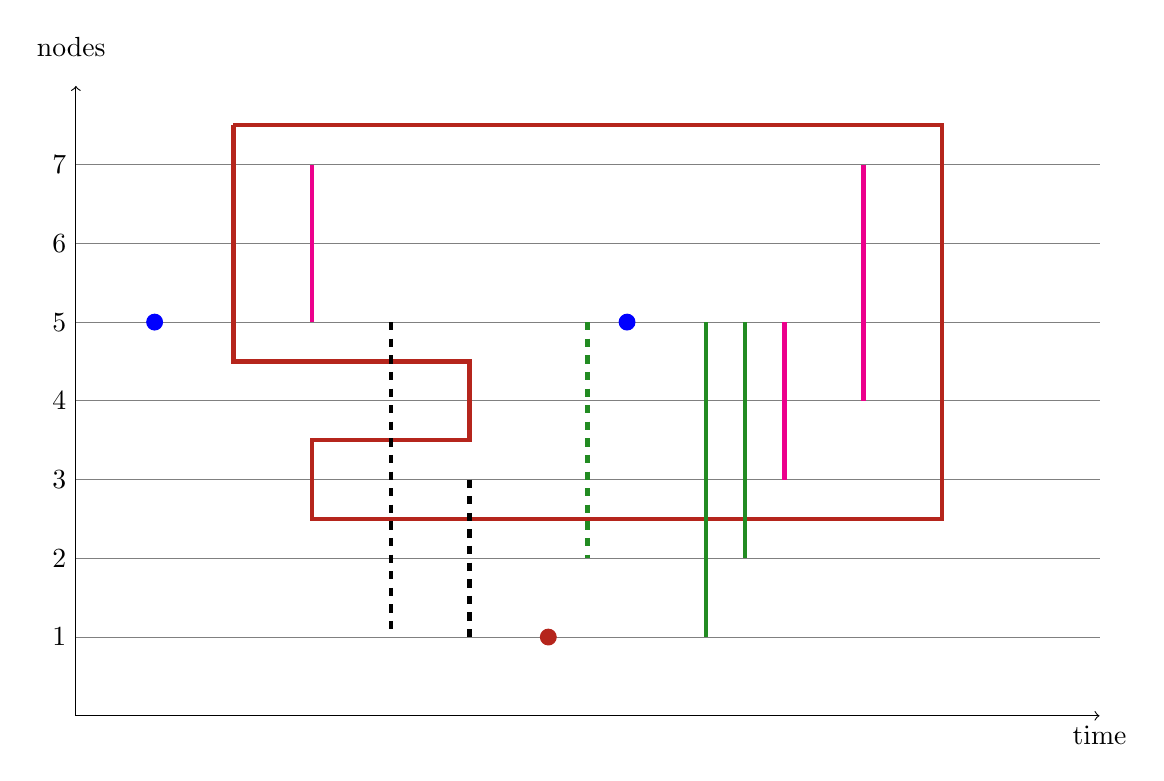
\begin{tikzpicture}

			\tikzstyle{comp outline}=[BrickRed, ultra thick]
			\tikzstyle{halo requests other comp}=[black, dashed, ultra thick]
			\tikzstyle{mig}=[blue, fill]
			\tikzstyle{deletion}=[BrickRed, fill]
			\tikzstyle{haloReqOptInt}=[ForestGreen, dashed, ultra thick]
			\tikzstyle{haloReqEnd}=[ForestGreen, ultra thick]
			\tikzstyle{coreReq}=[magenta, ultra thick]
		
		%axis
		\draw [<->] (1,6) -- (1,-2) -- (14,-2);
		\node [left, black] at (1,-1) {1};
		\node [left, black] at (1,0) {2};
		\node [left, black] at (1,1) {3};
		\node [left, black] at (1,2) {4};
		\node [left, black] at (1,3) {5};
		\node [left, black] at (1,4) {6};
		\node [left, black] at (1,5) {7};
		\node [left, black] at (1.5,6.5) {nodes};
		\node [below, black] at (14,-2) {time};
		
		
		%horizontal lines
		\draw [gray] (1,-1) -- (14,-1);
		\draw [gray] (1,0) -- (14,0);
		\draw [gray] (1,1) -- (14,1);
		\draw [gray] (1,2) -- (14,2);
		\draw [gray] (1,3) -- (14,3);
		\draw [gray] (1,4) -- (14,4);
		\draw [gray] (1,5) -- (14,5);
		
		%red component outline
		\draw [style = comp outline] (3,5.5) -- (3,2.5) -- (6,2.5) -- (6,1.5) -- (4,1.5) -- (4,0.5) -- (12,0.5) -- (12,5.5) -- (3,5.5);
		
		%core(C) edges
		\draw [coreReq] (4,3) -- (4,5);
		\draw [coreReq] (10,1) -- (10,3);
		\draw [coreReq] (11,2) -- (11,5);
		
		
		%blue points for opt migrations	
		\draw [mig] (8,3) circle [radius=0.1];
		\draw [mig] (2,3) circle [radius=0.1];		
		
		
		%green request lines for halo
		\draw [haloReqEnd] (9,3) -- (9,-1);
		\draw [haloReqEnd] (9.5,3) -- (9.5,0);
		
		
		%dashed green request lines for those assigned to an offline interval
		\draw [haloReqOptInt] (7.5,3) -- (7.5,0);
		
		
		%red dots for deletions of other components by crep
		\draw [deletion] (7,-1) circle [radius=0.1];
		
		%dashed black lines for requests assigned to other component
		\draw [halo requests other comp] (6,1) -- (6,-1);
		\draw [halo requests other comp] (5,3) -- (5,-1);	
		
		\end{tikzpicture}

		\centering
		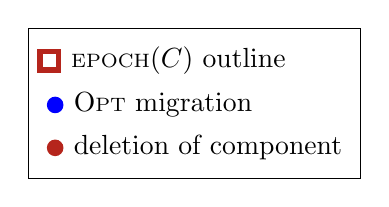
\begin{tikzpicture}[
			compOutline/.style={shape=rectangle, draw=BrickRed, line width=2},
			optMig/.style={shape = circle, fill=blue, inner sep=0pt,minimum size=6pt},
			optDel/.style={shape = circle, fill=BrickRed, inner sep=0pt,minimum size=6pt}]
			\matrix [draw,below left] at (10,0) {
			\tikzstyle{comp outline}=[BrickRed, ultra thick]
			\tikzstyle{halo requests other comp}=[black, dashed, ultra thick]
			\tikzstyle{mig}=[blue, fill]
			\tikzstyle{deletion}=[BrickRed, fill]
			\tikzstyle{haloReqOptInt}=[ForestGreen, dashed, ultra thick]
			\tikzstyle{haloReqEnd}=[ForestGreen, ultra thick]
			\tikzstyle{coreReq}=[magenta, ultra thick]
  \node [compOutline,label=right:\epoch($C$) outline] {}; \\
  \node [optMig,label=right:\opt{} migration]{};\\
  \node[optDel, label=right:deletion of component]{};\\
};
		\end{tikzpicture}
		\caption{Illustration of definitions used in the analysis; vertical lines 
		represent requests between the corresponding nodes; dashed black requests 
		are assigned to another component; the dashed green line is assigned to 
		the offline interval of node 5; the regular green lines are assigned to 
		an offline interval which is not contained in $\epoch(C)$}\label{analysis_def_illustration}
	\end{figure}
\end{center}

\begin{lemma}
	\label{offl_int_lemma}
	We assign at most $k\cdot\alpha$ requests from $N$ to any one offline interval.
\end{lemma}

\begin{proof}
	We fix an arbitrary offline interval of node $v$. Observe that none of the nodes involved in the assigned requests are moved by \opt{} during the offline interval, hence all the requests in question involve only nodes that \opt{} has placed on the same server as $v$ during the offline interval. 
	
	The number of such nodes is hence limited by the server capacity $k$. As we only examine requests from $\mathcal{H}$ we know that none of these requests have led \adjDel{} to perform any merges, hence there were at most $\alpha$ requests between $v$ and any one of the other nodes on its server during the offline interval. This bounds the number of requests assigned to the offline interval by $k\cdot\alpha$.
\end{proof}

Let $R(C)$ denote the set of requests from $\halo(C)\new{\backslash P}$ that were not assigned to any offline interval for a deleted component $C\in\del(\sigma)$ \new{and that \opt{} does not pay for}.
We say that a migration of node $v$ at time $t$ in the solution of \opt{} is \textit{contained} in $\epoch(C)$ if $(v,t)\in\epoch(C)$.
Let $\optmig(C)$ denote the cost of \opt{} due to migrations of nodes from component $C$ that are contained in $\epoch(C)$ and let $\optreq(C)$ denote the cost of \opt{} due to serving requests from $\core(C)$.
We show the following lower bound on the cost of \opt{} for migrations from $\optmig(C)$ and requests from $\optreq(C)$ for all deleted components $C$.

\begin{lemma}
	\label{opt_c_mig_req_lemma}
	\begin{align*}
	\sum_{C\in\del(\sigma)}\optmig(C)+\optreq(C)\geq 1/2\cdot\sum_{C\in\del(\sigma)} |C|/k\cdot\alpha+|R(C)|/k
	\end{align*}
\end{lemma}

\begin{proof}
	For the following part of the proof we fix an arbitrary component $C\in\del{}(\sigma)$. 
	Note that the nodes involved in requests from $R(C)$ were not moved by \opt{} during the processing of 
	requests from $R(C)$ until the time of deletion of $C$ as otherwise they would be assigned to an offline interval.
	
	The number of nodes contained in $C$ or connected to $C$ via edges representing requests 
	from $R(C)$ is at least $|C|+|R(C)|/\alpha$ since requests from $R(C)$ have not led 
	\adjDel{} to perform any migrations. Because of this fact \opt{} must have placed those nodes 
	on at least $\frac{|C|+|R(C)|/\alpha}{k}$ different servers. As \opt{} does not pay for any 
	requests from $R$ it follows that \opt{} must have placed the nodes from $C$ 
	in $(|C|+|R(C)|/\alpha)/ k$ different servers.
	
	We first examine the case in which \opt{} does not move any nodes from $C$ during $\epoch(C)$. 
	In this case \opt{} must partition a graph containing the nodes from $C$ which are connected 
	via edges representing the requests from $\core(C)$. As stated earlier \opt{} placed those 
	nodes in $(|C|+|R(C)|/\alpha)/ k$ different servers at time $\tau(C)$. 
	As \adjDel{} merged component $C$ this graph is $\alpha$-connected and hence \cref{cut_lemma} 
	gives that \opt{} has to cut at least edges of total weight 
	$((|C|+|R(C)|/\alpha)/ k)/2\cdot\alpha=1/2\cdot(|C|/k\cdot\alpha+|R(C)|/k)$.
	
	For the more general case in which \opt{} may perform node migrations during $\epoch(C)$ we 
	adapt the graph construction from above as follows: we add a vertex representing each 
	(node, time) pair from $\epoch(C)$.
	We connect each (node, time) pair $p$ with edges of weight $\alpha$ to the pairs of the same 
	node that represent the time step directly before and directly after $p$ (if they exist in 
	the graph). These edges represent the fact that \opt{} may choose to migrate a node between 
	any two time steps in $\epoch(C)$.
	Additionally we add an edge of weight one for each request $r=\{u,v\}$ from $\core(C)$ by 
	connecting the nodes in the graph that represent the pairs $(u,t)$ and $(v,t)$, respectively. 
	\opt{} once again has to partition this graph into $\frac{|C|+|R(C)|/\alpha}{k}$ parts.
	Note that we only added edges of weight $\alpha$ to the graph and hence this graph is 
	also $\alpha$-connected. We conclude that once again \opt{} has to cut edges of weight 
	at least $\frac{|C|+|R(C)|/\alpha}{k}\cdot1/2\cdot\alpha=1/2\cdot(|C|/k\cdot\alpha+|R(C)|/k)$.
	
	In both cases only edges representing either requests from $\optreq(C)$ or migrations 
	from $\optmig(C)$ were cut.
	As the sets $\core(C)$, $R(C)$ , $\core(D)$ and $R(D)$ are disjoint for two different 
	components $C,D\in\del(\sigma)$ per their definition we conclude that
	\begin{align*}
	\sum_{C\in\del(\sigma)}\optmig(C)+\optreq(C)\geq 1/2\cdot\sum_{C\in\del(\sigma)}|C|/k\cdot\alpha+|R(C)|/k.
	\end{align*}
\end{proof}


In the following lemma we combine the results of the previous lemmas in 
order to bound the cost of \opt{} given input sequence $\sigma$, 
denoted by $\opt(\sigma)$.


\begin{lemma}
	\label{opt_lower_bound}
	The cost of the solution of \opt{} given input sequence $\sigma$ is 
	bounded by
	\begin{align*}
	\opt{}(\sigma)\geq1/4\cdot\sum_{C\in\del{}(\sigma)}|C|/k\cdot\alpha+|\halo(C)|/k.
	\end{align*}
\end{lemma}

\begin{proof}
	We combine the results from \cref{offl_int_lemma} and 
	\cref{opt_c_mig_req_lemma}. Note that the cost from \cref{opt_c_mig_req_lemma} may 
	contain migration costs. In this case the corresponding migrations represent the end 
	of an offline interval. We denote the number of offline intervals by $o$. This gives 
	us that
	
	\begin{align*}
	2\opt{}(\sigma)\geq\sum_{C\in\del(\sigma)}\optmig(C)+\optreq(C)+ o\cdot\alpha+|P|
	\end{align*}
	as we account for each migration at most twice.
	
	Consider that due to \cref{offl_int_lemma} we have the inequality $o\geq|N|/k$. We repeat that $\mathcal{H}=\bigcup_{C\in\del{}(\sigma)}\halo{}(C)$. Note that $N$ is the subset of requests of $\mathcal{H}$ for which \opt{} does not pay while $P$ is the subset of $\mathcal{H}$ \opt{} pays for. It follows that the disjoint union of $N$ and $P$ is $\mathcal{H}$. Hence we obtain
	
	\begin{align*}
	2\opt{}(\sigma)&\geq\sum_{C\in\del(\sigma)}\optmig(C)+\optreq(C)+ o\cdot\alpha+|P|\\
	&\geq\sum_{C\in\del(\sigma)}1/2\cdot(|C|/k\cdot\alpha+|R(C)|/k)+(|N|+|P|)/k\\
	&\geq 1/2\cdot\sum_{C\in\del{}(\sigma)}|C|/k\cdot\alpha+|\halo(C)|/k.
	\end{align*}
	
This completes the proof.
\end{proof}


\subsection{Competitive Ratio}

We can now combine the results of \cref{crep_upper_bound} and \cref{opt_lower_bound} to obtain the following theorem which gives us the desired competitive ratio.

\begin{theorem}
	\label{comp_ratio_theo}
	With augmentation $(2+\epsilon)$ the competitive ratio of \adjDel{} is in $O(2/\epsilon\cdot k \log k)$.
\end{theorem}

\begin{proof}
	We arbitrarily fix an input sequence $\sigma$ and use our previous results to bound the competitive ratio of \adjDel{}. We define $\comps(\sigma):=\del{}(\sigma)\cup\finalComps(\sigma)$ in order to improve readability. Let $P$ denote the set of edges from $\bigcup_{C\in\del{}(\sigma)}\halo{}(C)$ that both \adjDel{} and \opt{} pay for.
	\begingroup
	\addtolength{\jot}{1em}
	\begin{align*}
	&\frac{\adjDel{}(\sigma)-\finalWeights(\sigma)}{\opt(\sigma)}\\ 
	&\leq\frac{2\cdot\sum_{C\in\comps(\sigma)}|C|\cdot((2/\epsilon+1)+\log k)\cdot\alpha +\sum_{C\in\del{}(\sigma)} |\halo(C)|}{1/4\cdot\sum_{C\in\del{}(\sigma)}|C|/k\cdot\alpha+|\halo(C)|/k +|P|}\\
	&\leq k \log k\frac{2\cdot\sum_{C\in\del(\sigma)}|C|\cdot(2/\epsilon+1) \cdot\alpha+\sum_{C\in\del{}(\sigma)}|\halo(C)|}{1/4\sum_{C\in\del{}(\sigma)}(|C|\cdot\alpha/2+|\halo(C)|)}+\beta\\
	& = O(2/\epsilon\cdot k \log k) +\beta
	\end{align*}
	\endgroup
	
	\noindent where
	\begin{align*}
	\beta=\sum_{C\in \finalComps(\sigma)}|C|\cdot((2/\epsilon+1)+\log k)\cdot\alpha
	\end{align*}
	
	\noindent Let $\beta'=\beta+\finalWeights(\sigma)$. Then it follows that
	
	\begin{align*}
	\frac{\adjDel{}(\sigma)}{\opt(\sigma)}\leq O(2/\epsilon\cdot k \log k) +\beta'.
	\end{align*}
	
	To obtain the bound on $\beta'$ we observe that the components in $\finalComps(\sigma)$ each are of size at most $k$ since they were not deleted by \adjDel{}. This allows us to derive the bound $\sum_{C\in \finalComps(\sigma)}|C|\cdot((2/\epsilon+1)+\log k)\leq \ell \cdot k \cdot ((2/\epsilon+1)+\log k)$. Since at the end of the execution of \adjDel{} there can be at most $k\cdot \ell$ components, \cref{cut_lemma_upper} allows us to bound $\finalWeights(\sigma)$ by $k\cdot \ell \cdot\alpha$. Hence we conclude that $\beta'\leq \ell\cdot k \cdot
	((2/\epsilon+1)+\log k)\cdot\alpha+k\cdot \ell\cdot \alpha\in O(2/\epsilon\cdot k \log k)$.
\end{proof}

\section{Polynomial-Time Implementation}
\label{implDetSection}

So far we have only shown that the algorithm \adjDel{} described in \cref{algIdeas} has a competitive ratio $O(2/\epsilon\cdot k \log k)$. 
We now show that it can also be implemented in polynomial time. 

In order to limit the section of the graph $G$ maintained by \adjDel{} that needs to be updated upon a new request between nodes of different components, we maintain a decomposition tree defined as follows: the root represents the whole graph and is assigned the connectivity of the entire graph. Given a node $v$ in the tree that represents a subgraph $G'$ of $G$, we decompose $G'$ into subgraphs whose connectivity is strictly larger than that of $G'$ and add children to $v$ for each such subgraph. We do not decompose sub-graphs of connectivity at least $\alpha$ any further as we only need to identify whether a new subgraph of connectivity at least $\alpha$ was created by the insertion of the most recent request.
Additionally we keep track of the connectivity of each such subgraph.
\cref{ex_decomp_tree} illustrates this decomposition for the graph shown in \cref{ex_graph}. In the decomposition tree we have labelled each node with the corresponding subset of vertices and the connectivity of the graph induced by these vertices.

If a new request is revealed to \adjDel{} then we only need to update the smallest subtree of the decomposition tree which still contains both end points of the request. 
This is correct because we can view each decomposition of a subgraph $G'$ into smaller graphs of a higher connectivity as a set of cuts that separates the nodes of $G'$. Inserting a new edge within a subgraph $G'$ may only increase the value of the cuts which result in the decomposition of $G'$, but do not affect cuts separating $G'$ itself from other subgraphs.
If a new request led to the creation of a new component this means that two old components that were at least $\alpha$-connected were merged and hence the number of leaves in the decomposition tree decreased. If this is the case then the algorithm checks whether the new component contains more than $k$ nodes. In this case the component is deleted and split into singleton components, each containing one node from the deleted component.

Upon such a component deletion the edges inside of and adjacent to the component are deleted, i.e. their weight is reset to zero. This means that the decomposition tree needs to be recomputed in order to reflect this change.
If however the resulting component $C$ contains at most $k$ nodes the algorithm tries to collocate the nodes of the component while minimizing migration costs, i.e. looking for a cluster which contains as many nodes of the newly merged component as possible but which also has enough free capacity for the remaining nodes to be moved there and for additional reservation $\min\{\lfloor\epsilon\cdot|C|\rfloor,k-|C|\}$.

%Both the decision whether to delete as well as possible node migrations are handled in the subroutine \textit{updateMapping} which is given the newly computed $\alpha$-connected components as input.

The detailed algorithms appear in Section
\ref{sec:detalg}.

\subsection{Subgraph Decomposition}
\label{decomp_desc}

We next describe our algorithm for the decomposition of a given subgraph represented by a node in the decomposition tree. 
%Specifically we describe the general idea behind our implementation of the subroutine \textit{decompose(treeNode, c)} which we have based on the algorithm described by Chang et al. (\cite{Chang2013}). In this algorithm $c$ denotes the connectivity that is the basis of this decomposition step.

Given a node $v$ of the decomposition tree, first a \textit{partition graph} is constructed which is a graph consisting of the nodes in the subgraph represented by $v$ and the edges which are between the nodes of the subgraph. This partition graph also supports merges and cuts of its nodes. More specifically the partition graph is initialized as a graph $P=(V,E)$ with $V=nodes(v)$ and $E=\{e=\{u,w\}\in E'|u\in nodes(v)\text{ and }w\in nodes(v)\}$ where $E'$ represents the set of edges in the graph maintained by \adjDel{}. Additionally we maintain a mapping $M$ which assigns each node from $V$ a set of the nodes in the subgraph represented by the decomposition tree node $v$. Initially M assigns each node in $V$ the subset containing only the node itself.

We now run a \textit{maximum adjacency search} algorithm, sometimes also called \textit{maximum cardinality search} algorithm \cite{Stoer1997}, in order to obtain an arbitrary minimum $(s,t)$-cut of the graph.
The maximum adjacency search algorithm is defined as follows: We start with an empty list $L$ to which we add an arbitrary node of $P$. We then continually add the most tightly connected node from $V$ to $L$, i.e. the node which is connected to the nodes in $L$ via edges of the most total weight. Stoer and Wagner \cite{Stoer1997} have shown that the edges between the last two nodes $s$ and $t$ added to $L$ form a minimum $(s,t)$-cut.
We use the value of this cut in order to decide whether to merge the nodes $s$ and $t$ or whether to separate them. If the cut has value less than $c$ we separate the nodes, otherwise we perform a merge.
Here the separation of the nodes $s$ and $t$ means that we remove all edges in the cut from the edges $E$ of the partition graph $P$.
In the case of a merge we combine the nodes $s$ and $t$ and merge the outgoing edges, i.e. we replace the set of nodes $V$ of $P$ by the set $V'=V\backslash\{s,t\}\cup\{v'\}$. The edges $E$ of $P$ are modified by removing all edges adjacent to $s$ and $t$ and adding an edge $e'=\{v',u\}$ of weight $w(\{s,u\})+w(\{t,u\})$ where $w(e)$ denotes the weight of edge $e$ if it exists and is equal to zero otherwise.
Furthermore we adjust the mapping $M$ by setting $M(v')=M(s)\cup M(t)$.

We continually run this algorithm until $P$ contains no edges, i.e. until $E=\emptyset$. The sets of nodes mapped to each ot the nodes of $P$ by $M$ now represent candidate subgraphs for the decomposition. Note though that we have only cut and merged according to minimum $(s,t)$-cuts and not according to minimum cuts. This means that the specific sequence in which we have performed the cuts may influence the result, e.g. if we merged based on a minimum $(s,t)$-cut which is not a minimum cut.
This can be remedied by repeating the procedure on the resulting subgraphs until it returns a subgraph of only one node, i.e. until no separation step is performed during the decomposition. This is due to the fact that this procedure always cuts a subgraph of connectivity less than $c$ at least once, as Chang et al. have shown (see Cutability Property in \cite{Chang2013}).
In order to speed up this computation we use the heap data structure proposed and analyzed by Chang et al. \cite{Chang2013}.

Thus we conclude that this procedure correctly decomposes a given subgraph as Chang et al. have also stated in Theorem 3.1 in \cite{Chang2013}.

%Next we discuss additional optimization ideas and then we show that this decomposition can be implemented in polynomial time.

There are several additional optimizations 
with which one can improve the running time of our implementation of \adjDel{}.
For example, with a $k$-core-based optimization, 
an $\alpha$-connected component 
	may only contain nodes or other components whose weighted degree is at least 
	$\alpha$. Hence we can iteratively cut all components whose weighted degree is 
	less than $\alpha$ until no more components can be cut by applying this rule.
Furthermore, we can track the smallest cut.
	In each decomposition step we keep track of the smallest minimum $(s,t)$-cut 
	that was encountered and then may increase the connectivity as maintained by 
	our decomposition tree data structure that corresponds to the current subgraph 
	to this number. This can significantly speed up our algorithm in cases where 
	parts of the tree are recomputed as it guarantees that each subtree is merged 
	completely at most once. For example there may be a case where after a deletion 
	of a component the connectivity of the whole graph is 0 but the graph still 
	contains large subgraphs of high connectivity. In this case the connectivity 
	of those subgraphs that is tracked in the tree can be increased by more than 
	one if a decomposition step has resulted in merges only.

\subsection{Running Time}
\label{run_time_sec}

We will now show that \adjDel{} is indeed a polynomial-time
algorithm.
The main bottleneck of the algorithm lies in the decomposition updates;
it is easy to see that 
the other parts of the algorithm can be implemented in polynomial time.

\begin{lemma}
	\label{dec_run_time_lem}
	The subroutine \textit{decompose} which decomposes a subgraph can be implemented in polynomial time $O(\alpha|V|^2|E|)$.
\end{lemma}

\begin{proof}
	The worst case is given when the whole tree has to be recomputed. We first discuss the time complexity of decomposing a single tree node $v$. Let the corresponding subgraph be denoted by $G_v=(V_v, E_v)$.
	Since each iteration of the subroutine \textit{decompose} performs at least one cut as long as the connectivity of the given graph is smaller than the current threshold $c$ we conclude that after at most $|V_v|$ iterations of decompose a correct decomposition is found. 
	
	Each step of \textit{decompose} can be performed in $O(|V_v|\cdot|E_v|)$ as the maximum adjacency search algorithm finds an arbitrary minimum $(s,t)$-cut in time $O(|E_v|)$ as shown in theorem 4.1 in \cite{Chang2013} and as there are at most $|V_v|$ minimum $(s,t)$-cuts computed for each invocation of \textit{decompose}.
	
	Hence the complexity of decomposing the subgraph represented by a tree node $v$ is in $O(|V_v|^2|E_v|)$. Let $C_v$ denote the time needed for the decomposition of the subgraph represented  by decomposition tree node $v$.
	
	We now sum this complexity over the nodes for each connectivity level of the decomposition tree. To this end let $level(i)$ denote all nodes in the decomposition tree which are of connectivity exactly $i$.
	
	\begin{align*}
	\sum_{i=0}^{\alpha}\sum_{v\in \text{level}(i)}C_v\leq\sum_{i=0}^{\alpha}O(|V|^2|E|)\in O(\alpha|V|^2|E|).
	\end{align*}
	
	We conclude our analysis of the time complexity by observing the polynomial-time complexity of $O(\alpha|V|^2|E|)$.
\end{proof}


We conclude our analysis of the running time by observing that the remaining subroutines can be implemented in polynomial time which results in the following theorem on the running time.

\begin{theorem}
	\label{run_time_theo}
	The algorithm \adjDel{} can be implemented in polynomial time.
\end{theorem}



\begin{comment}

\subsection{Comparison of \adjDel{} and \coreDel{}}

First we compare the results of \adjDel{} and \coreDel{}. \cref{costPlotCrep} shows the resulting total cost of both algorithms on the different input sets as well as how this cost is split between communication and migration costs. One can see that \adjDel{} always produces better results, especially for the second and third input set. 

We now discuss the differences of the two algorithms in terms of communication and migration cost. The figures illustrate that \adjDel{} pays only very slightly less for communication requests than \coreDel{} whereas the former pays significantly reduced migration cost. This suggests that the deletion of adjacent edges indeed improves the quality of the results by reducing the number of migrations. 

Finally \cref{runTimePlotCrep} compares the running times of both algorithms. One can see that \adjDel{} performs drastically better than \coreDel{} in this regard. This may be due to the fact that \adjDel{} deletes edges more frequently and thus needs to take less edges into account when updating the decomposition tree.

Also note that both algorithms generally pay more for migrations than for communication. This suggests that there may be room for fine-tuning these algorithms in order to achieve a more balanced distribution of the cost. One such adjustment is investigated in the next section, namely whether we can improve the results by changing the algorithms in such a way that they only merge once a connectivity of $2\cdot\alpha$ is reached.

\begin{figure}
	\begin{tikzpicture}
	\begin{axis}[
	ybar stacked,
	bar width=1cm,
	enlarge x limits=0.25,
	width=.45\textwidth,
	height=.5\textwidth,
	legend style={at={(0.5,-0.25)},
		anchor=north,legend columns=-1},
	symbolic x coords={\dbA,\dbB,\dbC},
	xtick=data,
	xlabel={input set},
	%nodes near coords,
	%nodes near coords align={vertical},
	ymajorgrids=true,
	ymin=0,ymax=370000,
	ylabel={cost},
	]
	\addplot table[x=database,y=AdjDel]{\commcostplot};
	\addplot table[x=database,y=AdjDel]{\migcostplot};
	
	\node[anchor=north west] at (rel axis cs:0,1) {\adjDel{}};
	%\legend{communication cost, migration cost}
	\end{axis}
	
	\begin{axis}[
	ybar stacked,
	bar width=1cm,
	enlarge x limits=0.25,
	width=.45\textwidth,
	height=.5\textwidth,
	legend style={at={(-0.2,-0.25)},
		anchor=north,legend columns=-1},
	symbolic x coords={\dbA,\dbB,\dbC},
	xtick=data,
	xlabel={input set},
	xshift=7cm,
	%nodes near coords,
	%nodes near coords align={vertical},
	ymajorgrids=true,
	ymin=0,ymax=370000,
	ylabel={cost},
	]
	\addplot table[x=database,y=CoreDel]{\commcostplot};
	\addplot table[x=database,y=CoreDel]{\migcostplot};
	\node[anchor=north west] at (rel axis cs:0,1) {\coreDel{}};
	\legend{communication cost, migration cost}
	\end{axis}
	\end{tikzpicture}
	\caption{Comparison of the total cost of \adjDel{} (left) and \coreDel{} (right)}\label{costPlotCrep}
\end{figure}

\begin{figure}
	\begin{tikzpicture}
	\begin{axis}[
	ybar=7pt,
	bar width=1.4cm,
	enlarge x limits=0.25,
	width=\textwidth,
	height=.5\textwidth,
	legend style={at={(0.5,-0.25)},
		anchor=north,legend columns=-1},
	symbolic x coords={\dbA,\dbB,\dbC},
	xtick=data,
	xlabel={input set},
	nodes near coords,
	nodes near coords align={vertical},
	ymin=0,ymax=700000,
	ylabel={time [ms]},
	]
	\addplot table[x=database,y=AdjDel]{\runtimeplot};
	\addplot table[x=database,y=CoreDel]{\runtimeplot};
	\legend{\adjDel{}, \coreDel{}}
	\end{axis}
	\end{tikzpicture}
	\caption{Comparison of running time of \adjDel{} and \coreDel{}}\label{runTimePlotCrep}
\end{figure}

\subsection{On the Influence of the Connectivity Threshold}
\label{alphaInf}

In the previous section we observed that both \coreDel{} and \adjDel{} have higher migration cost than communication cost. This leads to the question whether we can find adjustments that allow us to achieve a better balance of the different costs. In this section we investigate the influence of the connectivity threshold which determines when components are merged. Up until this point it was set to $\alpha$. As we show there lies potential in adjusting this threshold in order to improve the quality of the solution. 

Namely we discuss the results of both algorithms for the case where they only merge components once a connectivity of at least $2\cdot\alpha$ is reached. Note that this only affects the analysis by constant factors, namely the statements from \cref{cut_lemma} and \cref{cut_lemma_upper} are multiplied by a factor of two. This may only impact the other cost bounds by a factor of two which leaves our bound on the competitive ratio of \adjDel{} unaffected. Also note that we do not change the cost of a node migration, this cost is still $\alpha$.

\cref{costPlotCrepTwoAlpha} shows the total cost of \adjDel{} and \coreDel{} for this scenario. One can see that the costs of both algorithms are reduced, but \coreDel{} has improved significantly more than \adjDel{}.

When looking at the distribution of these costs to communication and migration costs one can see that now the communication costs of both algorithms are higher than the migration cost in all cases. For \coreDel{} this has improved the balance of both costs, but \adjDel{} now has significantly higher communication costs than migration costs. This suggests that by adjusting the exact value of connectivity at which these algorithms perform their merges one might be able to further improve the quality of the results. It may even be possible to adjust this parameter dynamically based on some data gathered as requests are processed.

These improvements come at a cost of running time as \cref{runTimePlotCrep2A} shows, almost doubling or tripling the times of the previous results in some cases. Especially the already worse run times of \coreDel{} are drastically increased.

\begin{figure}
	\begin{tikzpicture}
	\begin{axis}[
	ybar stacked,
	bar width=1cm,
	enlarge x limits=0.25,
	width=.45\textwidth,
	height=.5\textwidth,
	legend style={at={(0.5,-0.25)},
		anchor=north,legend columns=-1},
	symbolic x coords={\dbA,\dbB,\dbC},
	xtick=data,
	xlabel={input set},
	%nodes near coords,
	%nodes near coords align={vertical},
	ymajorgrids=true,
	ymin=0,ymax=370000,
	ylabel={cost},
	]
	\addplot table[x=database,y=AdjDelDouble]{\commcostplotTwoAlpha};
	\addplot table[x=database,y=AdjDelDouble]{\migcostplotTwoAlpha};
	\node[anchor=north west] at (rel axis cs:0,1) {\adjDel{}};
	%\legend{communication cost, migration cost}
	\end{axis}
	
	\begin{axis}[
	ybar stacked,
	bar width=1cm,
	enlarge x limits=0.25,
	width=.45\textwidth,
	height=.5\textwidth,
	legend style={at={(-0.2,-0.25)},
		anchor=north,legend columns=-1},
	symbolic x coords={\dbA,\dbB,\dbC},
	xtick=data,
	xlabel={input set},
	xshift=7cm,
	%nodes near coords,
	%nodes near coords align={vertical},
	ymajorgrids=true,
	ymin=0,ymax=370000,
	ylabel={cost},
	]
	\addplot table[x=database,y=CoreDelDouble]{\commcostplotTwoAlpha};
	\addplot table[x=database,y=CoreDelDouble]{\migcostplotTwoAlpha};
	\node[anchor=north west] at (rel axis cs:0,1) {\coreDel{}};
	\legend{communication cost, migration cost}
	\end{axis}
	\end{tikzpicture}
	\caption{Comparison of the total cost of \adjDel{} (left) and \coreDel{} (right) in the case where merges are performed at connectivity $2\cdot\alpha$}\label{costPlotCrepTwoAlpha}
\end{figure}


\begin{figure}
	\begin{tikzpicture}
	\begin{axis}[
	ybar=7pt,
	bar width=1.4cm,
	enlarge x limits=0.25,
	width=\textwidth,
	height=.5\textwidth,
	legend style={at={(0.5,-0.25)},
		anchor=north,legend columns=-1},
	symbolic x coords={\dbA,\dbB,\dbC},
	xtick=data,
	xlabel={input set},
	nodes near coords,
	nodes near coords align={vertical},
	ymin=0,ymax=1100000,
	ylabel={time [ms]},
	]
	\addplot table[x=database,y=AdjDelDouble]{\runtimeplotTwoAlpha};
	\addplot table[x=database,y=CoreDelDouble]{\runtimeplotTwoAlpha};
	\legend{\adjDel{}, \coreDel{}}
	\end{axis}
	\end{tikzpicture}
	\caption{Comparison of running time of \adjDel{} and \coreDel{} in the case where merges are performed at connectivity $2\cdot\alpha$}\label{runTimePlotCrep2A}
\end{figure}

\subsection{Results of \adapt{} and \static}

\begin{figure}
	\begin{tikzpicture}
	\begin{axis}[
	ybar stacked,
	bar width=1cm,
	enlarge x limits=0.25,
	width=.45\textwidth,
	height=.5\textwidth,
	legend style={at={(0.5,-0.25)},
		anchor=north,legend columns=-1},
	symbolic x coords={\dbA,\dbB,\dbC},
	xtick=data,
	xlabel={input set},
	%nodes near coords,
	%nodes near coords align={vertical},
	ymajorgrids=true,
	ymin=0,ymax=370000,
	ylabel={cost},
	]
	\addplot table[x=database,y=Adaptive]{\commcostplot};
	\addplot table[x=database,y=Adaptive]{\migcostplot};
	\node[anchor=north west] at (rel axis cs:0,1) {\adapt{}};
	%\legend{communication cost, migration cost}
	\end{axis}
	
	\begin{axis}[
	ybar stacked,
	bar width=1cm,
	enlarge x limits=0.25,
	width=.45\textwidth,
	height=.5\textwidth,
	legend style={at={(-0.2,-0.25)},
		anchor=north,legend columns=-1},
	symbolic x coords={\dbA,\dbB,\dbC},
	xtick=data,
	xlabel={input set},
	xshift=7cm,
	%nodes near coords,
	%nodes near coords align={vertical},
	ymajorgrids=true,
	ymin=0,ymax=370000,
	ylabel={cost},
	]
	\addplot table[x=database,y=Static]{\commcostplot};
	\addplot table[x=database,y=Static]{\migcostplot};
	\node[anchor=north west] at (rel axis cs:0,1) {\static{}};
	\legend{communication cost, migration cost}
	\end{axis}
	\end{tikzpicture}
	\caption{Comparison of the total cost of \adapt{} (left) and \static{} (right)}\label{costPlotMetis}
\end{figure}



\cref{costPlotMetis} shows the total cost of the solutions of \adapt{} and \static{}. One can see that \static{} is able to produce results that far surpass \adapt{}. In fact the results of \static{} are also a significant improvement over the results of \adjDel{} and \coreDel{} presented before. But it is also important to note that \static{} is only useful in scenarios where the communication patterns and frequencies stay mostly the same over time. Otherwise the approach to record the communication graph and then use \static{} in order to compute a partitioning may lead to inconsistent results. 

We stress that the implementations of \static{} and \adapt{} rely on heuristics only and do not provide any guarantees while we have shown that our algorithm \adjDel{} is a competitive algorithm with competitive ratio $O(2/\epsilon\cdot k\log k)$.

Finally \cref{runTimePlotMetis} illustrates the run times of \adapt{} and \static{}. Note that static is only run once on the communication graph after all requests have been revealed which means that it is expected for \static{} to have the fastest running time. But also \adapt{} achieves faster running times than our dynamic implementations.

\begin{figure}[h]
	\begin{tikzpicture}
	\begin{axis}[
	ybar=7pt,
	bar width=1.4cm,
	enlarge x limits=0.25,
	width=\textwidth,
	height=.5\textwidth,
	legend style={at={(0.5,-0.25)},
		anchor=north,legend columns=-1},
	symbolic x coords={\dbA,\dbB,\dbC},
	xtick=data,
	xlabel={input set},
	nodes near coords,
	nodes near coords align={vertical},
	ymin=0,ymax=150000,
	ylabel={time [ms]},
	]
	\addplot table[x=database,y=Adaptive]{\runtimeplot};
	\addplot table[x=database,y=Static]{\runtimeplot};
	\legend{\adapt{}, \static{}}
	\end{axis}
	\end{tikzpicture}
	\caption{Comparison of running time of \adapt{} and \static{}}\label{runTimePlotMetis}
\end{figure}
\end{comment}

\section{Related Work}
\label{sec:related_work}

The closest work to ours is by Avin et al. \cite{Avin2015} 
who initiated the study of the dynamic balanced graph partitioning 
problem. The authors present a $O(k \log k)$-competitive algorithm 
with augmentation $2+\epsilon$ for any $\epsilon>1/k$;
this algorithm however has a super-polynomial runtime,
which we improve upon in this paper.  
In their paper, Avin et al. also show a lower bound of $k-1$ for the competitive ratio of any online algorithm 
on two clusters via a reduction to online paging. 
Restricted variants of the balanced repartitioning problem have also been studied. Here one assumes certain restrictions of the input sequence $\sigma$ and then studies online algorithms for these cases. 
Avin et al. \cite{Avin2018} 
assume that an adversary provides requests according to a fixed distribution of which the optimal algorithm \opt{} has knowledge while an online algorithm that is compared with \opt{} has not. Further the authors restrict the communication pattern to form a ring-like pattern, i.e. for the case of $n$ nodes $0,...,n-1$ only requests $r$ of the form $r=\{i \mod n, (i+1)\mod n\}$ are allowed. For this case they present a competitive online algorithm which achieves a competitive ratio of $O(\log n)$ with high probability.	
Henzinger et al. \cite{Henzinger2019} 
study a special \textit{learning variant} of the problem 
where it is assumed that the input sequence $\sigma$ eventually reveals a perfect balanced partitioning of the $n$ nodes into $\ell$ parts of size $k$ such that the edge cut is zero. In this case the communication patterns reveal connected components of the communication graph of which each forms one of the partitions. Algorithms are tasked to \textit{learn} this partition and to eventually collocate nodes according to the partition while minimizing communication and migration costs.
The authors of \cite{Henzinger2019} present an algorithm for the case where the number of servers is $\ell=2$ that achieves a competitive ratio of $O((\log n)/\epsilon)$ with augmentation $\epsilon$, i.e. each server has capacity $(1+\epsilon)n/2$ for $\epsilon\in(0,1)$.
For the general case of $\ell$ servers of capacity $(1+\epsilon)n/\ell$ the authors construct an exponential-time algorithm that achieves a competitive ratio of $O((\ell\log n \log \ell)/\epsilon)$ for $\epsilon\in(0,1/2)$ and also provide a distributed version.
Additionally the authors describe a polynomial-time $O((\ell^2\log n\log \ell)/\epsilon^2)$-competitive algorithm for the case with general $\ell$, servers of capacity $(1+\epsilon)n/\ell$ and $\epsilon\in(0,1/2)$.

The dynamic balanced graph partitioning problem 
can be seen as a generalization (or symmetric version) of online paging.
In the online paging problem \cite{Fiat2002}, \cite{Epstein2011}
 one is given a scenario with a fast cache of $k$ pages and $n-k$ pages in slow memory. Pages are requested in an online manner, i.e. without prior knowledge of future requests. If a requested page is in the cache at the time of the request it can be served without cost. If it is in slow memory however, then a \textit{page fault} occurs and the requested page needs to be moved into the cache. If the cache is full then a page from the cache needs to be evicted, i.e. moved to the slow memory in order to make space for the requested one. The goal is to design algorithms which minimize the number of such page faults.
However, the standard version of online paging has no equivalent to the option of serving a request remotely as is possible in the Dynamic Balanced Graph Partitioning problem. The variant \textit{with bypassing} allows an algorithm to access pages in slow memory without moving them into the cache, thus providing such an equivalent. It is worth stressing however that in our problem requests involve two nodes while in Online Paging the nodes themselves are requested.

The static balanced graph partitioning problem is the static offline variant of the problem of this paper. In this version an algorithm may not perform any migrations, but has perfect knowledge of the request sequence $\sigma$ and then needs to provide a perfectly balanced partitioning of the $n=k\cdot \ell$ nodes into $\ell$ sets of equal size $k$ that minimizes cost, i.e. the weight of edges between the servers. This scenario can be modelled as a graph partitioning problem where the weight of an edge corresponds to the number of requests between its end points in the input sequence $\sigma$. 
An algorithm then has to provide a partition of the nodes into sets of exactly $k$ nodes each while minimizing the total edge weights between partitions, i.e. an algorithm needs to minimize the edge cut of the graph.  
This problem is NP-complete (\cite{Andreev2006}) and for the case where $\ell\geq 3$, Andreev and R\"acke \cite{Andreev2006} have shown that there is no polynomial time approximation algorithm which guarantees a finite approximation factor unless P=NP.

There are several algorithms and frameworks for graph partitioning problems. Usually these frameworks employ heuristics in order to achieve their results. The most successful such heuristic is \textit{Multilevel Graph Partitioning} \cite{Buluc2016}. This method consists of three phases. Initially the graph is repeatedly coarsened into a hierarchy of smaller graphs in such a way that cuts in the coarse graphs also correspond to cuts in the finer graphs. On the coarsest level a (potentially expensive) algorithm is used in order to compute an initial partition. This partitioning is then transferred to the finer graphs. In this process one usually uses other local heuristics in order to improve the partition quality even further with every step.
METIS \cite{Karypis1998, Karypis1998a} and Jostle \cite{Walshaw2000, walshaw2007jostle} are examples of libraries that utilize this multilevel approach. We choose METIS as a reference for our empirical evaluation.

More generally, clustering has been studied within a variety of
different contexts 
from data mining to image segmentation \cite{Benabdellah2019, Wu1993, Pavana},
and is the process of generating subsets of elements with high similarity 
\cite{Hartuv2000}. 
However, we consider an online problem, i.e. algorithms need to react dynamically to changes in the graph and need to maintain their data structures and adapt accordingly whereas clustering considers complete data sets which are static.

\section{Future Work}
	\label{sec:future_work}
	
While our algorithm does not only achieve a polynomial runtime
and an almost competitive ratio (up to a logarithmic factor),
our work leaves upon several interesting directions for future
research. 
On the theoretical front, it would be interesting to explore
how to close the gap between upper and lower bound
on the competitive ratio, and to study randomized algorithms.
On the practical front, we believe that our algorithm can
be further engineered and optimized to achieve a lower runtime
in practice, as well as an improved empirical competitive ratio
under real (non worst-case) workloads.
These kinds of adjustments may be achieved for example by changing certain algorithm parameters such as the connectivity threshold.
There may also be potential in adapting and improving our decomposition tree data structure in order to improve running times.
%Finally, we plan to provide a distributed implementation 


\bibliography{../bibtex/ThesisBibTex}


\appendix
%%
%% Bibliography
%%

%% Please use bibtex, 

\section{Deferred Technical Details}

\subsection{Preliminaries: Adaptions from \cite{Avin2015}}\label{sec:preli}

\begin{lemma}
	\label{mergeableLemma}
	At any time $t$ after \adjDel{} performed its merge and delete actions, all subsets $S$ of components with $|S|>1$ have connectivity less than $\alpha$, i.e. there exist no mergeable component sets after \adjDel{} performed its merges and deletions.
\end{lemma}
\begin{proof}
	We prove the lemma by induction. The lemma holds trivially at time 0.
	Now assume that at some time $t>0$ the lemma does not hold, i.e., there is a subset $S$ of components with connectivity at least $\alpha$ and $|S|>1$. We may assume that $t$ is the earliest time for which $S$ has connectivity $\alpha$.
The incrementation of the weight of some edge $e$ at time $t$ raised the connectivity of $S$, but $S$ was not merged into a new $\alpha$-connected component $C$. If no new component was created at time $t$ we arrive at a contradiction as \adjDel{} always merges if there exists a mergeable component set.
	
	Now assume that a component $C$ was created at time $t$. This means that $C$ must also contain the endpoints of $e$. But then the conjunction of $C$ and $S$ forms an even larger subset of components with connectivity at least $\alpha$ which is a contradiction to the maximality of $C$ and $S$.
\end{proof}

The following lemma is adapted for our connectivity-based approach from Corollary 4.2 in \cite{Avin2015}.

\begin{lemma}
	\label{mergeable_lemma}
	Fix any time $t$ and consider weights right after they were updated by \adjDel{} but before any merge or delete actions. Then all subsets $S$ of components with $|S|>1$ have connectivity at most $\alpha$ and a mergeable component set $S$ has connectivity exactly $\alpha$.
\end{lemma}

\begin{proof}
	This lemma follows directly from \cref{mergeableLemma} as connectivities can only increase by at most 1 at each time $t$ and \cref{mergeableLemma} guarantees that mergeable component sets are merged by \adjDel{} directly after they emerge before a new request is revealed.
\end{proof}

The following two lemmas combined give us a result similar to Lemma 4.3 in \cite{Avin2015}: bounds on the edge weight that is cut when partitioning a mergeable component set, i.e. a set of components of connectivity at least $\alpha$.

We start by establishing a lower bound on this edge weight in the following lemma.

\begin{lemma}
	\label{cut_lemma}
	Given a mergeable set of components $S$ and a partition of $S$ into $g>1$ parts $S_1,...,S_g$. Then the weight between the parts of the partition is at least $g/2 \cdot \alpha$.
\end{lemma}

\begin{proof}
	We construct a graph $G$ with the different parts $S_i, i\in\{1,...,g\}$ of the partition as nodes. Note that this graph is $\alpha$-connected. We insert an edge for each edge between the parts $S_i$. Now consider the sum of the weighted degrees of all such nodes $S_i$ in the constructed graph:
	\begin{align*}
	\sum_{i\in\{1,...,g\}}deg_G(S_i)=2\sum_{e\in G}w(e)
	\end{align*}
	The equality follows as the left sum counts each edge twice, once for each endpoint.
	Now consider the fact that each node $S_i$ must have degree at least $\alpha$ with respect to the edges in $G$ because $G$ is $\alpha$-connected. Hence
	\begin{align*}
	2\sum_{e\in G}w(e)=\sum_{i\in\{1,...,g\}}deg_G(S_i)\leq\sum_{i\in\{1,...,g\}}\alpha=g\cdot\alpha
	\end{align*}
	which gives us that $\sum_{e\in G}w(e)\geq g/2\cdot\alpha$.
\end{proof}

In the following lemma we establish the upper bound on the cut edge weight when partitioning a mergeable set of components $S$ into $g\geq2$ parts.

\begin{lemma}
	\label{cut_lemma_upper}
	Given a mergeable set of components $S$ and a partitioning of $S$ into $g\geq2$ parts $S_1,...,S_g$. The weight between the parts $S_i$ is at most $(g-1)\cdot\alpha$ during the execution of \adjDel{}.
\end{lemma}

\begin{proof}
	Similarly to before we construct a graph $G=(V,E)$ with the different parts $S_i, i\in\{1,...,g\}$ of the partition as nodes and we insert an edge for each edge between the parts $S_i$. Note again that this graph is $\alpha$-connected. We iteratively partition $G$ into subsets via minimum cuts with regard to edge weight, i.e. we consider a minimum edge cut of $G$ which partitions the nodes of $G$ into the subsets $V_1$ and $V_2$. We continue to iteratively partition the resulting sets until all sets contain only one node of $G$ each. As this required at most $|V|-1$ cuts of value at most $\alpha$ and $|V|=g$ by definition of $G$ the lemma follows.
\end{proof}

\begin{center}
	\begin{figure}	
		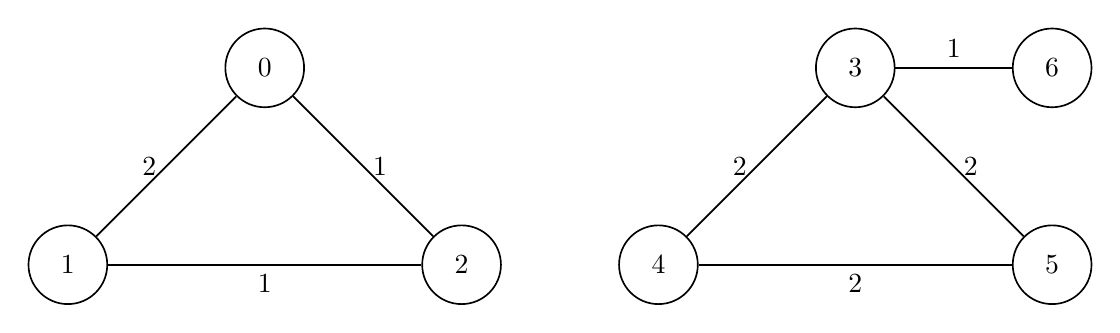
\begin{tikzpicture}[-latex ,auto ,node distance =2.5 cm and 2.5cm ,on grid ,
		semithick ,
		state/.style ={ circle ,top color =white , bottom color = white ,
			draw, black , text=black , minimum width =1 cm}]
		\node[state] (A) {$0$};
		\node[state] (B) [below left =of A] {$1$};
		\node[state] (C) [below right =of A] {$2$};
		\node[state] (E) [right =of C]{$4$};
		\node[state] (D) [above right =of E] {$3$};		 
		\node[state] (F) [below right =of D] {$5$};
		\node[state] (G) [right =of D]{$6$};
		\path (A) edge[-] node[left] {$2$} (B); % 0 to 1
		\path (A) edge[-] node[right] {$1$} (C); % 0 to 2
		\path (B) edge[-] node[below] {$1$} (C); % 1 to 2
		\path (D) edge[-] node[left] {$2$} (E); % 3 to 4
		\path (D) edge[-] node[right] {$2$} (F); % 3 to 5
		\path (E) edge[-] node[below] {$2$} (F); % 4 to 5
		\path (D) edge[-] node[above] {$1$} (G); % 3 to 6
		\end{tikzpicture}
		\caption{Example graph}
		\label{ex_graph}
	\end{figure}
\end{center}

\begin{figure}
	\Tree[.{$\{0,1,2,3,4,5,6\}$\\conn$=0$} 	[.{$\{0,1,2\}$\\conn$=2$} 	[.{$\{0\}$\\conn$=\infty$} ]
	[.{$\{1\}$\\conn$=\infty$} ]
	[.{$\{2\}$\\conn$=\infty$} ]]
	[.{$\{3,4,5,6\}$\\conn$=1$} [.{$\{3,4,5\}$\\conn=4} ]
	[.{$\{6\}$\\conn$=\infty$} ]]]
	
	\caption{Decomposition tree for the graph from \cref{ex_graph} for $\alpha=4$}
	\label{ex_decomp_tree}
\end{figure}

\begin{algorithm}
	\caption{insertAndUpdate($a$,$b$)}
	\label{insertAndUpdate}
	\begin{algorithmic}
		\IF {comp[$a$] == comp[$b$]}
		\STATE return
		\ENDIF
		\STATE addEdge($a,b$)
		\STATE updateDecomposition$(a,b)$
		\STATE $del\leftarrow$ updateMapping$(alphaConnectedComponents)$
		\STATE delComponents$(del)$
	\end{algorithmic}
\end{algorithm}

\subsection{Detailed Algorithms}
\label{sec:detalg}

We now present our algorithms in more details.
\cref{insertAndUpdate} is the main function that is called upon each new request. It checks whether the new request is between different $\alpha$-connected components. If this is not the case it determines that this request cannot change the decomposition and returns.
Otherwise the weight of the corresponding edge is increased and other routines are called that update the decomposition based on this new edge.
\cref{updateDecomposition} first determines the smallest sub-graph in the decomposition tree that contains both end points of the request and decomposes this sub-graph. For this decomposition step we use the algorithm proposed by Chang et al. \cite{Chang2013}. We explain this algorithm in greater detail in \cref{decomp_desc}.

\begin{algorithm}
	\caption{updateDecomposition($a$,$b$)}
	\label{updateDecomposition}
	\begin{algorithmic}
		\STATE $q\leftarrow$ findSmallestSubgraph$(a,b)$
		\WHILE{$q$ not empty}
		\STATE current$\leftarrow$ $q$.popFront()
		\IF{$res$.connectivity==$\alpha$}
		\STATE continue
		\ENDIF
		\STATE $res\leftarrow$ decompose(current, current.connectivity+1) // 
		\emph{decomposition based on $(s,t)$-cuts} 
		\STATE current.connectivity $\leftarrow$ value of smallest encountered cut
		\IF {current.connectivity$\geq\alpha$}
		\STATE continue
		\ENDIF
		\STATE childrenQueue $\leftarrow res$
		\STATE //make sure that only subgraphs with higher connectivity are added as children
		\WHILE{childrenQueue not empty}
		\STATE $c\leftarrow$childrenQueue.pop()
		\STATE $cRes\leftarrow$decompose($c$, current.connectivity+1)
		\STATE $c$.connectivity $\leftarrow$ value of smallest encountered cut
		\IF{decompose returned only one graph}
		\STATE current.children.add($cRes$)
		\IF{$cRes$ has connectivity smaller than $\alpha$}
		\STATE $q$.push($cRes$)
		\ENDIF
		\ELSE
		\STATE childrenQueue.add($cRes$)
		\ENDIF
		\ENDWHILE
		\ENDWHILE
	\end{algorithmic}		
\end{algorithm}

Afterward, the routine \textit{updateMapping} is called which compares the number of components to the number of components before the arrival of the request. Only if the number of components has decreased, it checks for the new component; otherwise there was no component merge. 
If there was a merge then the routine examines the size of the newly created (merged) component and decides whether to delete or to collocate based on the logic described in the previous section.

If a deletion has to be performed, then this step is done in the routine \textit{delComponents} (\cref{delComponents}) which resets all edge weights both of edges between nodes of the component as well as all adjacent edges and finally starts the decomposition of the whole graph in order to arrive at a new decomposition that follows the definition from the previous section.
In the case of a collocation, the nodes are moved to a cluster that has enough space while updating the reservations and cluster capacities accordingly.



\begin{algorithm}
	\caption{delComponents($del$)}
	\label{delComponents}
	\begin{algorithmic}
		\STATE delAllEdges($del$)
		\STATE root.connectivity=0
		\STATE root.children=\{\}
		\STATE updateDecomposition(0,1)
	\end{algorithmic}
\end{algorithm}

\section{Empirical Evaluation}
\label{sec:evaluation}

In order to complement our analytical results and shed light
on the performance of our algorithm in practice, 
we implemented $\adjDel$ and conducted experiments
under real-world traffic traces from datacenters
and high-performance computing clusters. 
We also discuss an algorithm engineering approach to improve the practical
performance of $\adjDel$, and compare the algorithm to different reference algorithms
and heuristics.

\subsection{Reference Algorithms}
\label{algSection}

We compare our algorithm based on maintaining a second-order partition of the nodes into components we discussed in \cref{algIdeas}, 
i.e. \adjDel{} where on a component deletion all edges inside of and adjacent to the component are deleted, with reference algorithms. 
We have shown the competitive ratio of \adjDel{} in \cref{comp_ratio_theo} and its polynomial running time in the previous section.

We consider the following baselines in our evaluation.
First, we consider an alternative implementation 
of \adjDel{}, called \directDecomp{}, that does not use the decomposition tree 
	structure mentioned in \cref{implDetSection}.
	Rather, this implementation 
	applies the MinCut-based decomposition algorithm presented in \cref{decomp_desc}
	to the whole graph and thus computes the new components in one decomposition step.

Furthermore, recall that \adjDel{} always maintains a second-order partition of the nodes 
into components, and when a component is deleted, all edges inside of and adjacent to the component are reset. 
A natural alternative, is to reset internal edges only on this occasion;
we will refer to this algorithmic variant as $\coreDel$.
The \adjDel{} and $\coreDel$ 
algorithms start with randomly initialized mappings of nodes to servers.

Another natural reference algorithm is a static graph partitioning;
to this end, we use the METIS\_PartGraphRecursive algorithm 
implemented in the METIS framework \cite{Karypis1998, Karypis1998a},
and will refer to it simply as \static{}. %Both frameworks are known to produce very good results and to be very fast.
For \static{} we first record the communication graph resulting
from the requests, and give it as input to \static{}. 
We then compute the cost of \static{} due to migrations from the random initial mapping of nodes to servers; in addition, we charge 
the remote requests, i.e. the total weight of edges between nodes of the communication graph which \static{} mapped to different servers.
The algorithms start with randomly initialized mappings of nodes to servers.

\subsection{Traffic Traces and Methodology}
\label{inputDesc}

\begin{figure}
	\begin{center}
		\begin{tabular}{|l|c|c|c|c|c|c|}
			\hline
			trace & nodes & requests & $\ell$ & $k$ & $\alpha$ & $\epsilon$\\
			\hline
			\dbnekbone{} & 512 & 250 000 & 32 & 16 & 3 & 0.1 \\
			\dbmocfe{} & 1024 & 250 000 & 32 & 32 & 3 & 0.1 \\
			\fb{} & 2048 & 10 000 & 64 & 32 & 3 & 0.1 \\
			\hline
		\end{tabular}
	\end{center}
	\caption{Traffic traces used in the evaluation}
	\label{fig:trace_overview}
\end{figure}

We consider different real-world traffic traces (workloads),
two hpc traces, \dbnekbone{} and \dbmocfe{}, as well as a trace from 
a Facebook data center which we call \fb{}.
 The traces and their characteristics 
are described in more detail in \cite{Avin2019}.
The traces are publicly available.

With \dbmocfe{} we study a scenario 
where the number of servers is $\ell=32$, each of size $k=32$, and 
we use the first 250k requests in a setting with 1024 nodes. 
For \fb{} we restrict the trace to 2048 nodes. For this restriction we 
 iteratively chose the vertex pairs that communicate the most during the first 20 million requests 
until we reached the number of 2048 nodes; we 
then added all requests between two of these nodes to our data set. 
For this scenario, we used a configuration with $\ell=64$ 
servers is $\ell=32$ of size $k=32$.
The runs are then performed on the first 10k of these requests. Similarly we  restricted \dbnekbone{} to 512 nodes and 
used the first 250k requests for this setting; 
this data set is then evaluated in a scenario where the number of servers is $\ell=32$, each of size $k=32$.
For all configurations we use $\alpha=3$ and $\epsilon=0.1$.
These configurations are summarized in \cref{fig:trace_overview}.
The influence of $\alpha$ on the running time is investigated further in \cref{sec:alpha_influence}.

\subsection{Runtime Evaluation}

We evaluate the running time of \adjDel{} by considering different traces 
and alternative algorithms. 
	\begin{figure}[ht]
		\centering
		\begin{minipage}{0.48\linewidth}
			\begin{subfigure}[b]{\linewidth}
				\includegraphics*[width=\linewidth]{new_time_all_filtered_decompTree}
				\caption{time results for \adjDel}
			\end{subfigure}		
		\end{minipage}
		\begin{minipage}{0.48\linewidth}
			\begin{subfigure}[b]{\linewidth}
				\includegraphics*[width=\linewidth]{new_time_all_filtered_compDecomp}
				\caption{Runtime results for \directDecomp}
			\end{subfigure}		
		\end{minipage}
		\begin{subfigure}[b]{0.48\linewidth}
			\includegraphics*[width=\linewidth]{new_time_all_filtered_coreDel}
			\caption{Runtime results for \coreDel{}}
		\end{subfigure}
		\caption{Comparison of the runtimes of \adjDel{} (top left), \directDecomp{} (top right) and \coreDel{} (bottom) for all 3 data sets}\label{fig:all_runtimes_boxplot}
	\end{figure}

\cref{fig:all_runtimes_boxplot} shows the results of all data sets for \adjDel{} and \directDecomp{}.  Here
we filtered the running times to only include updates which have led the respective algorithm to update, i.e. those updates where the communicating nodes belonged to different components at the time of the request. 
We can see that for all three algorithms \fb{} produces by far the longest runtime and that \directDecomp{} performs significantly better than \adjDel{} and \coreDel{} for \fb{}.
We first compare the runtimes of the three algorithms for the hpc data sets before we discuss the runtimes for \fb{} in greater detail.

\begin{figure}
	\centering
	\begin{minipage}{0.48\linewidth}
		\begin{subfigure}[b]{\linewidth}			\includegraphics*[width=\linewidth]{new_time_hpc_filtered_decompTree}
			\caption{Runtime results for \adjDel}
		\end{subfigure}		
	\end{minipage}
	\begin{minipage}{0.48\linewidth}
		\begin{subfigure}[b]{\linewidth}
			\includegraphics*[width=\linewidth]{new_barplot_time_hpc_filtered_decompTree}
			\caption{Total time for \adjDel}
		\end{subfigure}		
	\end{minipage}
	\begin{minipage}{0.48\linewidth}
		\begin{subfigure}[b]{\linewidth}
			\includegraphics*[width=\linewidth]{new_time_hpc_filtered_compDecomp}
			\caption{Runtime results for \directDecomp}			
		\end{subfigure}		
	\end{minipage}
	\begin{minipage}{0.48\linewidth}
		\begin{subfigure}[b]{\linewidth}
			\includegraphics*[width=\linewidth]{new_barplot_time_hpc_filtered_compDecomp}
			\caption{Total time for \directDecomp}
			
		\end{subfigure}		
	\end{minipage}
	\begin{minipage}{0.48\linewidth}
		\begin{subfigure}[b]{\linewidth}
			\includegraphics*[width=\linewidth]{new_time_hpc_filtered_coreDel}
			\caption{Runtime results for \coreDel{}}
		\end{subfigure}		
	\end{minipage}
	\begin{minipage}{0.48\linewidth}
		\begin{subfigure}[b]{\linewidth}
			\includegraphics*[width=\linewidth]{new_barplot_time_hpc_filtered_coreDel}
			\caption{Total time for \coreDel{}}
		\end{subfigure}		
	\end{minipage}
	\caption{Comparison of the runtimes of \adjDel{} (top), \directDecomp{} (middle) and \coreDel{}(bottom) for both hpc traces}\label{fig:hpc_runtimes_boxplot_restricted}
\end{figure}

\cref{fig:hpc_runtimes_boxplot_restricted} shows plots of run times of \adjDel{}, 
\directDecomp{} and \coreDel{} for the HPC traces. On the left of the figure you can see the 
distribution of the update times over the requests while the total times are shown 
on the right. The figure shows that \adjDel{} is the fastest for both hpc traces while \coreDel{}
is faster than \directDecomp{}. This indicates that the decomposition tree data 
structure which both \adjDel{} and \coreDel{} use may be a significant advantage 
for the HPC traces.

\begin{figure}
	\begin{minipage}{0.48\linewidth}
		\begin{subfigure}[b]{\linewidth}
			\includegraphics*[height=7cm]{plot_facebook_time_to_size}
			\caption{Relation of size to time for \fb{} for \adjDel{}}
		\end{subfigure}		
	\end{minipage}
	\begin{minipage}{0.48\linewidth}
		\begin{subfigure}[b]{\linewidth}
			\includegraphics*[height=7cm]{plot_facebook_time_to_size_coreDel}
			\caption{Relation of size to time for \fb{} for \coreDel{}}
		\end{subfigure}		
	\end{minipage}
	
	\caption{Relation of size to time for \fb{} for \adjDel{} (left) and \coreDel{} (right)}\label{fig:fb_size_to_time}
\end{figure}

\cref{fig:fb_size_to_time} illustrates the relation of the time needed 
for handling a 
request, and the number of edges in the data structure for \adjDel{} and for \coreDel{} for \fb{}. 
We can see a high correlation, i.e. a large number of edges in the graph maintained by 
the respective algorithm seems to lead to longer update times. Similarly the update times are shorter after 
the number of edges decreases, i.e. after a component deletion. 
While we cannot prove this, we suspect that this may 
be due to the fact that the data used for the run shows little structure, 
and thus leads
a large number of (costly) recomputation steps for our data structure. This is also supported 
by the fact that \directDecomp{} is significantly faster for \fb{} as one can see in 
\cref{fig:all_runtimes_boxplot}.

\label{sec:alpha_influence}
\begin{figure}[ht]
	\begin{minipage}{0.48\linewidth}
		\begin{subfigure}{\linewidth}
			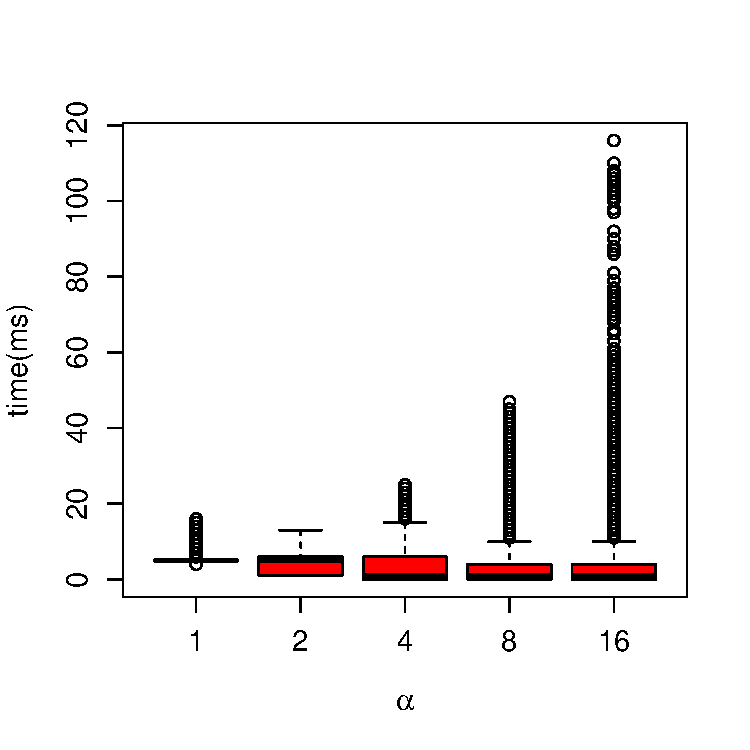
\includegraphics[height=6cm]{boxplot_varying_alphas_mocfe_decompTree}
			\caption{Runtime of \adjDel{} for \dbmocfe{} for different values of $\alpha$}
		\end{subfigure}				
	\end{minipage}
\begin{minipage}{0.48\linewidth}
	\begin{subfigure}{\linewidth}
		\includegraphics*[height=6cm]{plot_varying_alphas_mocfe}
		\caption{Total runtime of \adjDel{} for \dbmocfe{} for different values of $\alpha$}
	\end{subfigure}
\end{minipage}
	\begin{minipage}{0.48\linewidth}
		\begin{subfigure}{\linewidth}
			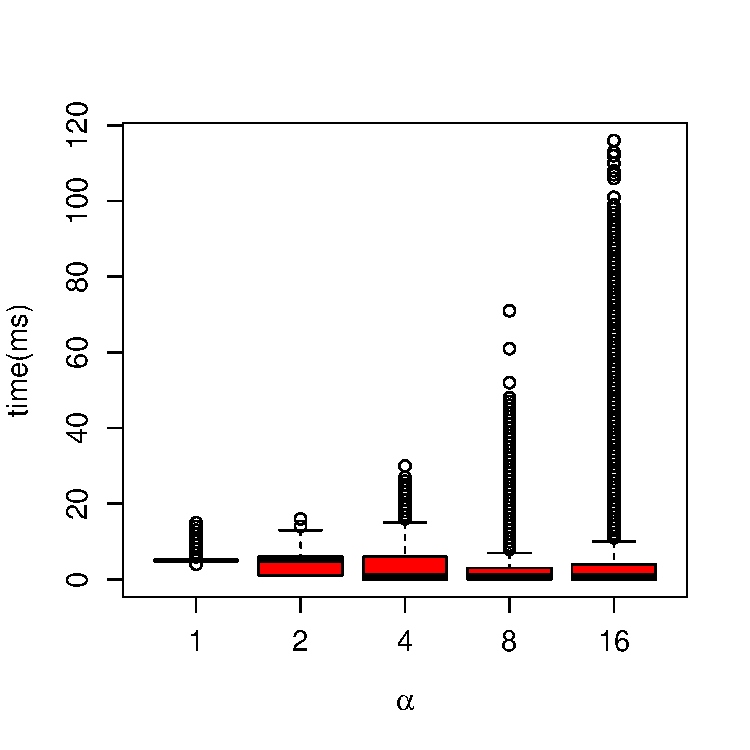
\includegraphics[height=6cm]{boxplot_varying_alphas_mocfe_coreDel}
			\caption{Runtime of \coreDel{} for \dbmocfe{} for different values of $\alpha$}
		\end{subfigure}				
	\end{minipage}
	\begin{minipage}{0.48\linewidth}
		\begin{subfigure}{\linewidth}		
			\includegraphics*[height=6cm]{plot_varying_alphas_mocfe_coreDel}
			\caption{Total runtime of \coreDel{} for \dbmocfe{} for different values of $\alpha$}
		\end{subfigure}	
	\end{minipage}	
	
	\caption{Runtime of \adjDel{} (top) and \coreDel{} (bottom) for \dbmocfe{} for different values of $\alpha$}
	\label{fig:alpha_influence}
\end{figure}

It is also interesting to study 
the influence of $\alpha$ on the running time of \adjDel{} and \coreDel{}.
\cref{fig:alpha_influence} shows a plot of the running time of \adjDel{} for $\alpha\in\{1,2,4,8,16\}$. In order to improve the readability,
only requests which led to an update of the data structure are included. The results show that \adjDel{} is slower for $\alpha=1$ than for $\alpha\in\{2,4\}$.
This may be due to the fact that lower values of $\alpha$ lead \adjDel{} to 
update the tree structure more frequently.
Especially for $\alpha=1$ every inserted edge leads to a merge, as edges are only inserted between different components and $\alpha$ 
is both the cost for a node migration as well as the connectivity threshold for merging for \adjDel{}.
The remaining results mirror the expectation that the increase in the potential height of the decomposition tree also increases the required time 
as the update times may increase.

\subsection{Cost Evaluation}

In order to shed light on the cost, in terms of communication 
and migration, we compare our algorithms \adjDel{} and \coreDel{} with \static{}.

\begin{figure}[ht]
	\centering
	\begin{minipage}{0.48\linewidth}
		\begin{subfigure}[b]{\linewidth}
			\includegraphics*[width=\linewidth]{plot_cost_decompTree}
			\caption{Cost of \adjDel}
		\end{subfigure}		
	\end{minipage}
	\begin{minipage}{0.48\linewidth}
		\begin{subfigure}[b]{\linewidth}
			\includegraphics*[width=\linewidth]{plot_cost_coreDel}
			\caption{Cost of \adjDel}
		\end{subfigure}
	\end{minipage}
	\begin{subfigure}[b]{0.48\linewidth}
		\includegraphics*[width=\linewidth]{plot_cost_static}
		\caption{Cost of \static{}}
	\end{subfigure}	
	\caption{Comparison of the costs of \adjDel{} (left), \coreDel{} (right) and \static{} (bottom) for all 3 data sets}\label{fig:all_cost_barplot}
\end{figure}

\cref{fig:all_cost_barplot} shows the costs of \adjDel{}, \coreDel{} and \static{} for \fb{}, \dbmocfe{} and \dbnekbone{}.
Note that for \fb{} the costs of \adjDel{} and \coreDel{} are actually lower than the cost of \static{}. For the HPC traces
\static{} is able to achieve significantly lower cost than both \adjDel{} and \coreDel{}.
However, keep in mind that \static{} is essentially an offline algorithm,
which knows requests ahead of time; furthermore, we also note that 
\static{} may not produce a perfectly balanced partitioning.

\end{document}
